%!TEX root = ../thesis.tex
%*******************************************************************************
%****************************** Third Chapter **********************************
%*******************************************************************************
\chapter{The dynamic sRNA profile and inheritance of paternal epigenetic modifications post-fertilisation in the embryo of \textit{Marchantia polymorpha}}

% **************************** Define Graphics Path **************************
\ifpdf
    \graphicspath{{Chapter3/Figs/Raster/}{Chapter3/Figs/PDF/}{Chapter3/Figs/}}
\else
    \graphicspath{{Chapter3/Figs/Vector/}{Chapter3/Figs/}}
\fi


\section{Abstract}

Global cytosine methylation reprogramming has recently been reported in the male sexual lineage of \textit{Marchantia polymorpha}. During spermiogenesis, global 5mC expansion occurs, followed by the expansion of 4mC onto CG sites. Following fertilisation, the mature embryo loses this epigenetic mark. Therefore, the fate of paternal N4-methylcytosine methylation is explored in early \textit{Marchantia} embryos. The results suggest that 4mC is actively removed prior to pronuclear fusion. This is further corroborated by exploring the phenotype of embryos fertilised by 4mC knockout sperm using fluorescent reporter lines, which exhibit accelerated embryonic development and a partial fertility cost.


\section{Introduction}

As discussed in Chapter 1, DNA methylation is an important epigenetic modification in both prokaryotes and eukaryotes. In eukaryotes the most prevalent DNA modification is 5mC, important in gene regulation, imprinting, silencing TEs and responding to environmental stimuli. In prokaryotes, in addition to 5mC, additional base modifications, such as N6-methyladenine (6mA) and 4mC are also present and play key roles in restriction-modification systems and in marking self DNA to distinguish it from foreign DNA (Figure \ref{fig:base_mods}) \cite{RN309}.

\begin{figure}[htbp!] 
\centering    
    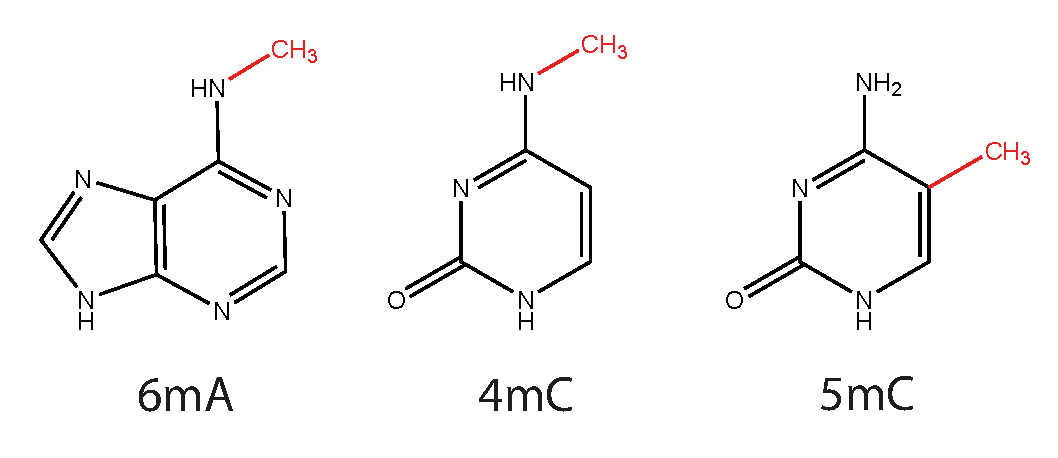
\includegraphics[width=0.5\textwidth]{Chapter3/Figs/Intro/base_mods.pdf}
\caption{Eukaryotic and prokaryotic base modifications}
\label{fig:base_mods}
\captionsetup{font=small}
    \caption*{}
\end{figure}

DNA methylation reprogramming during sexual development is a common feature in eukaryotes. As discussed in previous chapters, the epigenetic reprogramming in the male sexual lineage of \textit{Arabidopsis} is extensive and is a characteristic shared by other flowering plants. However, given that male sexual lineage development and meiosis in \textit{Arabidopsis} occur within a few cell divisions (Figure \ref{fig:male_sex_dev}), our group aimed to investigate whether gene-targeted methylation is specifically associated with meiosis or spermiogenesis.

The lifecycle of the basal land plant \textit{Marchantia polymorpha} alternates between haploid and diploid phases. In the haploid vegetative phase (thallus), they can reproduce asexually or be induced by far-red light to produce gametophytes. These gametophytes form antheridiophores (which produce antheridia and sperm in males) and archegoniophores (which produce archegonia and egg cells in females). Once the egg cell is fertilised by sperm, \textit{Marchantia} proceeds to go through a rapid diploid sporophytic phase, which culminates in meiosis and the dispersal of haploid spores (Figure \ref{fig:Mp_lifecycle}) \cite{RN143}.

\begin{figure}[htbp!] 
\centering    
    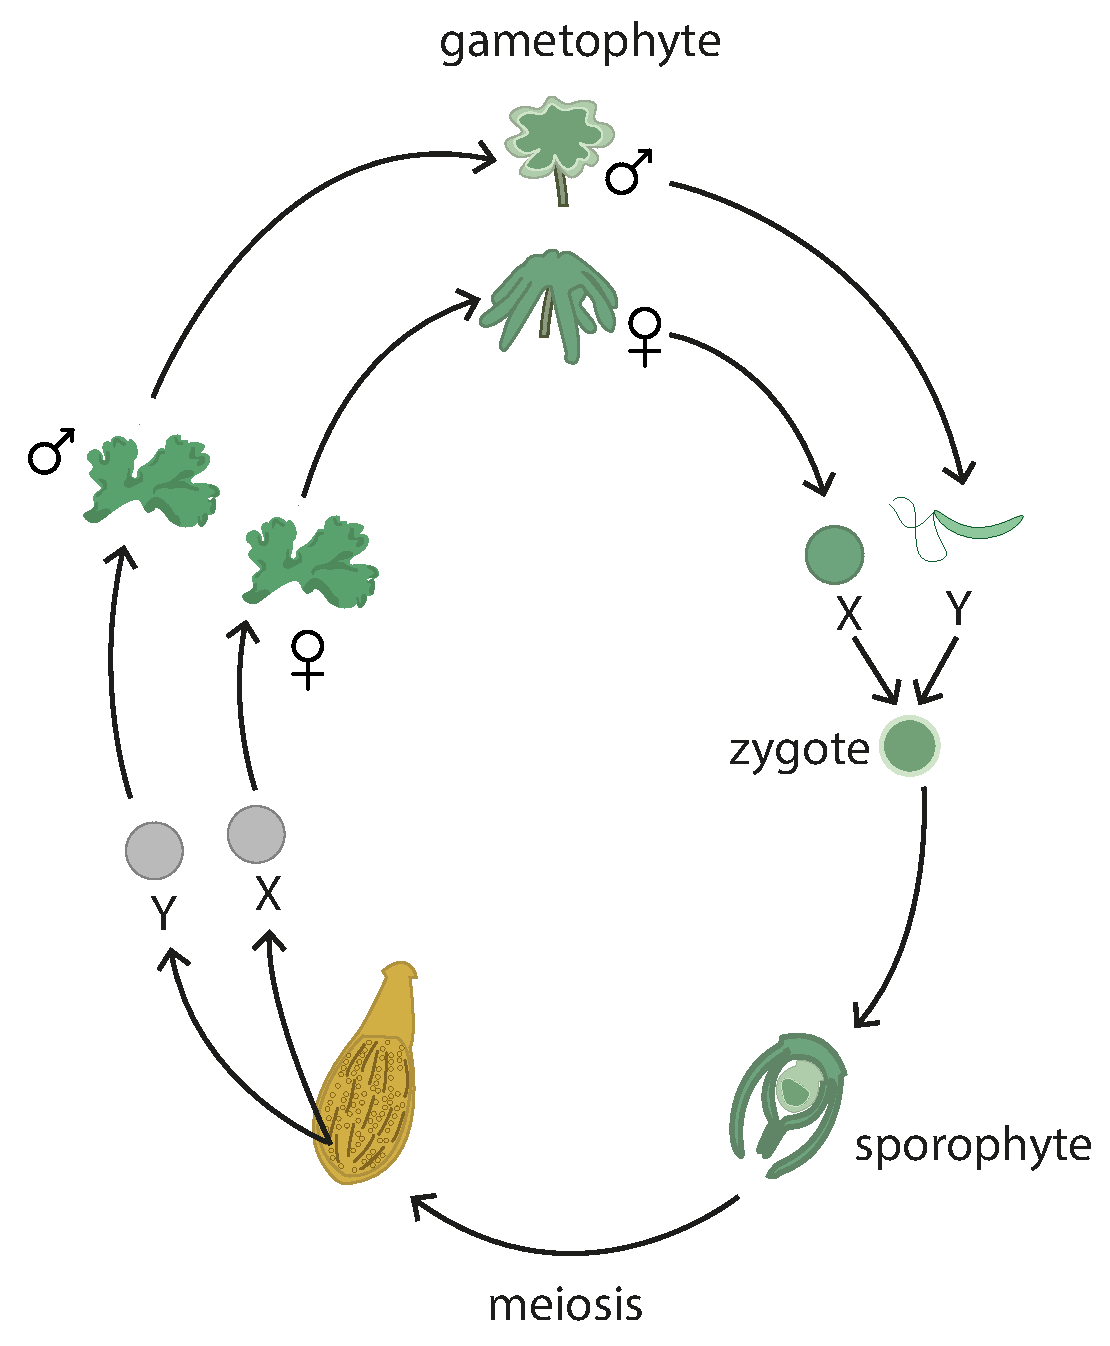
\includegraphics[width=0.7\textwidth]{Chapter3/Figs/Intro/Marchantia_lifecycle.pdf}
\caption{The lifecycle of \textit{Marchantia polymorpha}}
\label{fig:Mp_lifecycle}
\captionsetup{font=small}
    \caption*{}
\end{figure}

Recently, our group demonstrated that during spermiogenesis in \textit{Marchantia}, there is extensive DNA methylation reprogramming. In addition to the deposition of 5mC, a second wave of DNA methylation reprogramming occurs, involving the deposition of N4-methylcytosine (4mC) — an epigenetic modification previously thought to exist only in prokaryotes — at the majority of CG sites across the genome (Figure \ref{fig:Mp_graphical_abstract}). A 4mC methyltransferase, MpDN4MT1, was identified as the enzyme catalysing genome-wide 4mC methylation. Knockout of the \textit{dn4mt1} gene results in the loss of 4mC, partial fertility defects, and impaired sperm motility \cite{RN189}.

\begin{figure}[htbp!] 
\centering    
    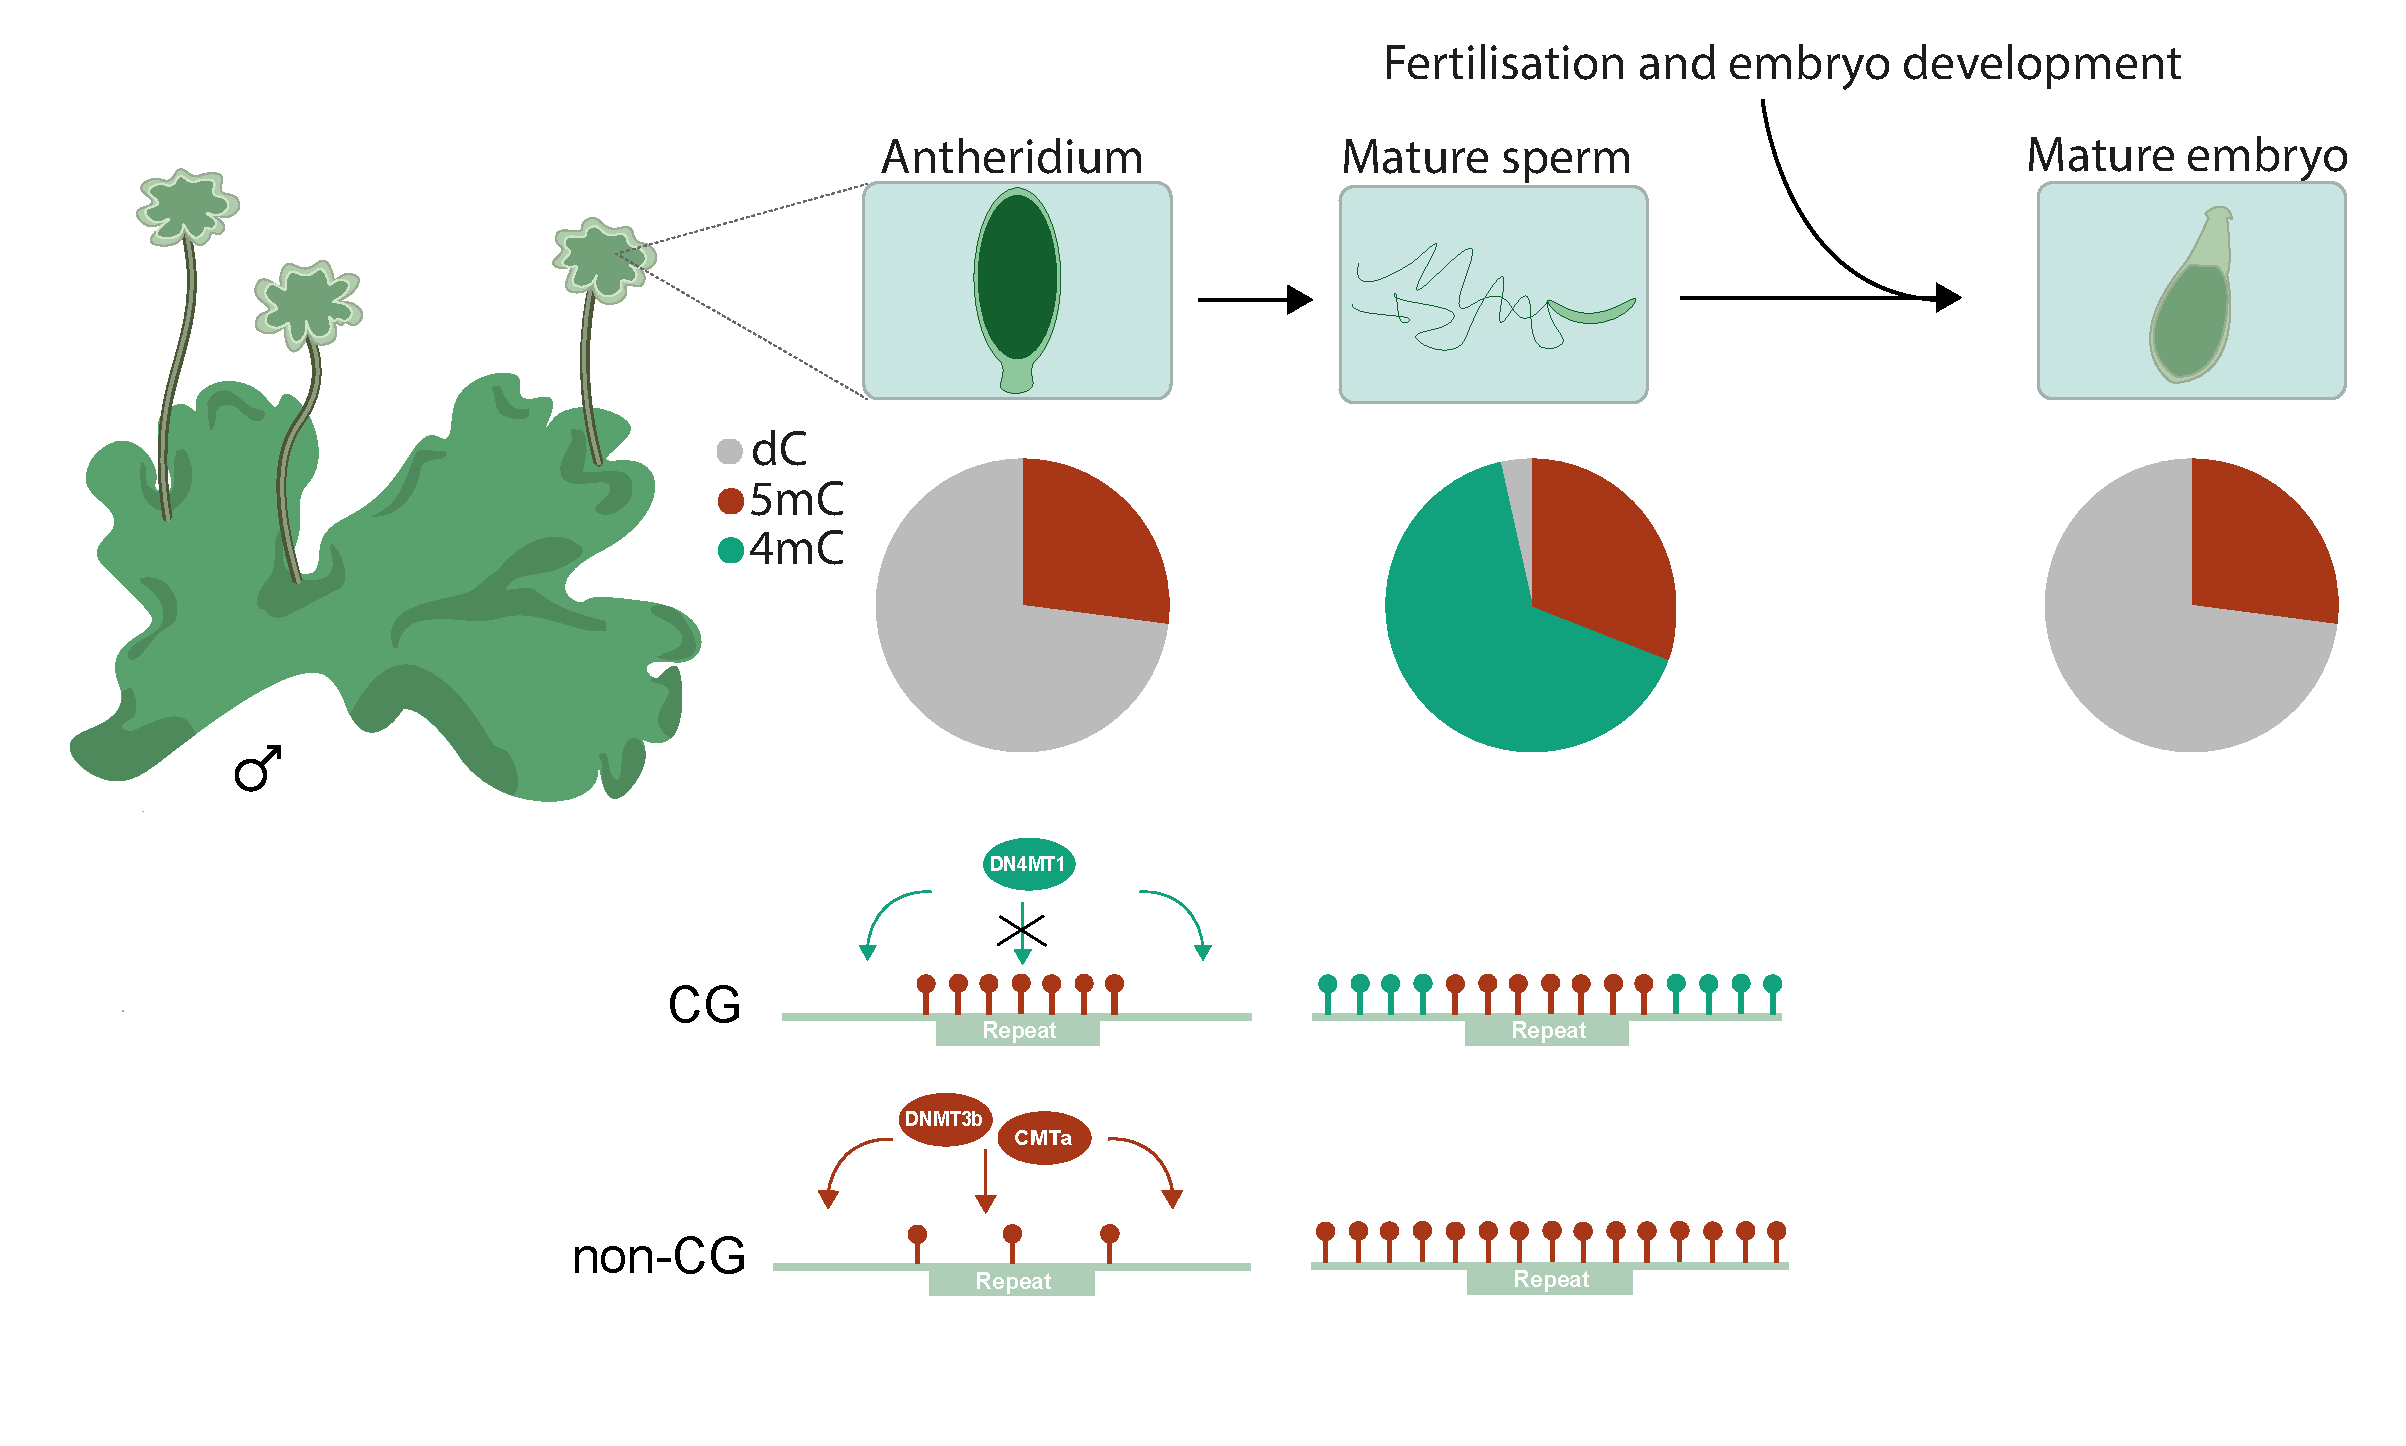
\includegraphics[width=1\textwidth]{Chapter3/Figs/Intro/Graphical_abstract.pdf}
\caption{The landscape of DNA methylation during the spermiogenesis and embryogenesis of \textit{Marchantia}}
\label{fig:Mp_graphical_abstract}
\captionsetup{font=small}
    \caption*{In the liverwort \textit{Marchantia polymorpha }it was recently reported \cite{RN189} that during spermiogenesis, two waves of DNA methylation reprogramming occur. First 5mC is deposited (brown) facilitated by DNA methyltransferases DNMT3b and CMTa followed by a dramatic second wave, wereby 4mC expands to genic regions to cover the majority of CG sites in sperm (green), catalysed by a novel methyltransferase MpDN4MT1. Following fertilisation,  4mC methylation is lost in the embryo. Figure adapted from \cite{RN189}.}
\end{figure}

Paternal 4mC methylation is absent in the mature embryo (which contains over 1000 cells). The exact timing of when 4mC methylation is lost post-fertilisation remains unknown, as does whether the paternal genome retains any 4mC marks during the early stages of zygotic development. In \textit{Marchantia}, the first division of the zygote occurs approximately 3–4 days after fertilisation (DAF) \cite{RN139}, suggesting that 4mC may need to be actively removed for pronuclear fusion to take place. This hypothesis aligns with the observed phenotype where embryos fertilised by \textit{dn4mt1} sperm exhibit accelerated development (Figure \ref{fig:burstpeak}, data collected by dr Yalin Liu), though this phenomenon still requires confirmation during early embryonic stages. Alternatively, 4mC methylation could be lost passively following fertilisation through dilution by cell division, or actively removed post-fertilisation for DNA replication or cell division to function normally. Additionally, 4mC may play a role in ensuring correct genome dosage and transcriptional activity during early embryonic development.

\begin{figure}[htbp!] 
\centering    
    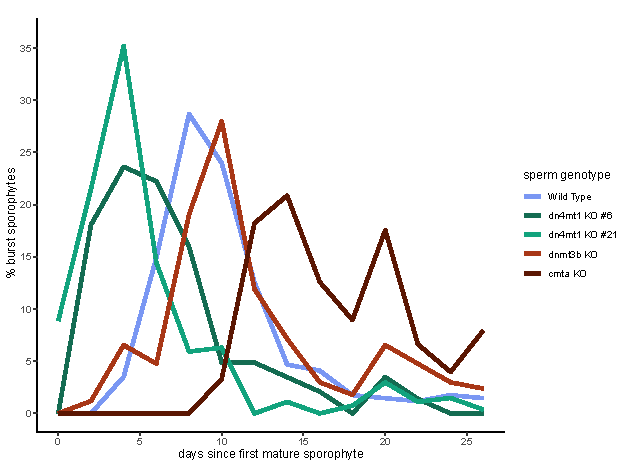
\includegraphics[width=1\textwidth]{Chapter3/Figs/Intro/burstpeak_nuclei_number.pdf}
\caption{Embryos fertilised by \textit{dn4mt1} knockout sperm develop more rapidly than WT}
\label{fig:burstpeak}
\captionsetup{font=small}
    \caption*{Total percentage of burst sporophytes every day since first mature sporophyte, fertilised with wild type sperm (blue), two independent lines of \textit{dn4mt1} knockout sperm (\#6 dark green, \#21 light green) or 5mC (\textit{cmta} (dark brown) or \textit{dnmt3B}) knockout sperm (light brown). Data collected by dr Yalin Liu.}
\end{figure}

In \textit{Arabidopsis}, 5mC methylation is actively removed to maintain homeostasis through the action of several DNA glycosylases. \textit{Arabidopsis} encodes four DNA demethylases: DEMETER (DME), REPRESSOR OF SILENCING 1 (ROS1), and the DEMETER-LIKE proteins DML2 and DML3. While DME is involved in vegetative cell demethylation in pollen \cite{RN57} (as discussed in Chapter 2), it also plays a critical role in the allele-specific expression of maternally imprinted genes in the central cell and endosperm \cite{RN235}. The remaining DNA glycosylases appear to be functionally redundant, primarily preventing the spread of transposon-derived 5mC methylation into genic regions\cite{RN288}, including ROS1 \cite{RN168}. Therefore, the orthologs of ROS1 in \textit{Marchantia}, MpROS1a and MpROS1x (located on the female sex chromosome) offer possible candidates for erasing paternal 4mC methylation as they are expressed in the sperm \cite{RN212} and mature eggs/embryos \cite{RN257} respectively \cite{RN169,RN257,RN189}.

Recent findings have shown that the heterochromatic histone modification H3K27me3 is exclusively deposited on the paternal genome during the pronuclear stage of the embryogenesis of \textit{Marchantia}, leading to the repression of the paternal genome, which persists throughout embryogenesis \cite{RN160}. In contrast, in mammalian germlines, H3K27me3-mediated imprinting is limited to a few loci within the female gamete \cite{RN172}. 4mC therefore offers a possible mechanism through which the paternal genome could be marked during early development.

Hence, investigating the methylation profiles of early \textit{Marchantia} embryos during the first zygotic divisions and examining the early developmental phenotype of \textit{dn4mt1} mutants complement our previous work, expanding our understanding of how paternal DNA methylation affects early embryonic development.

\clearpage

\section{Paternal 4mC is lost in the early embryo of \textit{Marchantia}}

To establish an effective method for staging early \textit{Marchantia} embryos and identify the earliest feasible window for embryo extraction for AMD sequencing (AMD-seq), several approaches were explored. Despite incorporating detergents, vacuum-assisted staining, and testing various stains (DAPI, Hoechst 33342, and ethidium bromide), live-cell staining of developing embryos within the archegonium remained inconsistent. This inconsistency likely arises from the embryo's position within a cavity (the venter) surrounded by somatic cells and cell walls (Figure \ref{fig:egg_embryo} rows one and two). Moreover, variations in environmental conditions during embryo development significantly impacted growth, as illustrated in Figure \ref{fig:embryo_diff} which shows the same genotype embryos 10 days post-fertilisation under different growth conditions. To ensure consistency and reproducibility, a controlled crossing method was adopted, wherein archegoniophores were exposed to sperm in a tube for an hour, ensuring synchronised fertilisation and uniform embryo development. This approach is particularly suited for studying early embryo development, as embryos can be cultured under these conditions for up to two weeks \cite{RN139}. Under these conditions, the earliest developing embryos could be manually dissected was around 7–8 days after fertilisation (Figure \ref{fig:egg_embryo}).

\begin{figure}[htbp!] 
\centering    
    \includegraphics[width=1\textwidth]{Chapter3/Figs/Figure1_eggs_and_embryos.pdf}
\caption{Live cell imaging of the developmental stages of \textit{M. polymorpha} embryos}
\label{fig:egg_embryo}
\captionsetup{font=small}
    \caption*{Unstained egg cell (first row), DAPI stained egg cell (second row), and embryos 8 days (third row), and 10 days (fourth row) after fertilisation. Scale bar 10$\mu$m}
\end{figure}

As previously established, 4mC methylation is deposited in the CG context over gene bodies and outside TEs during spermiogenesis by MpDN4MT1 (Figure \ref{fig:ends_analysis}A)\cite{RN189}. Although 5mC methylation across all sequence contexts over TEs increases during germline development, non-CG methylation is specifically deposited during spermiogenesis by MpCMTa and MpDNMT3B (Figure \ref{fig:ends_analysis}B,D and F)\cite{RN189}. Additionally, this methylation pattern is deposited and maintained over gene bodies (excluding the transcription start site, TSS), with 4mC serving as the primary methylation mark at the TSS. 

As early embryos are difficult to harvest, first AMD-seq (sequencing specifically 4mC) and EM-seq (sequencing specifically 5mC) was tested on wild type sperm and compared to data previously collected from wild type sperm and \textit{dn4mt1} sperm (Figure \ref{fig:ends_analysis} WT sperm rep2 AMD-seq (light green) and \textit{dn4mt1} sperm AMD-seq (grey)). The expected methylation patterns over genes and TEs in the 4mC and 5mC contexts were confirmed by the sperm AMD-seq and EM-seq libraries (Figure \ref{fig:ends_analysis} wild type sperm rep2 AMD-seq (light green), wild type sperm EM-seq (dark brown).) 

\begin{figure}[htbp!] 
\centering    
    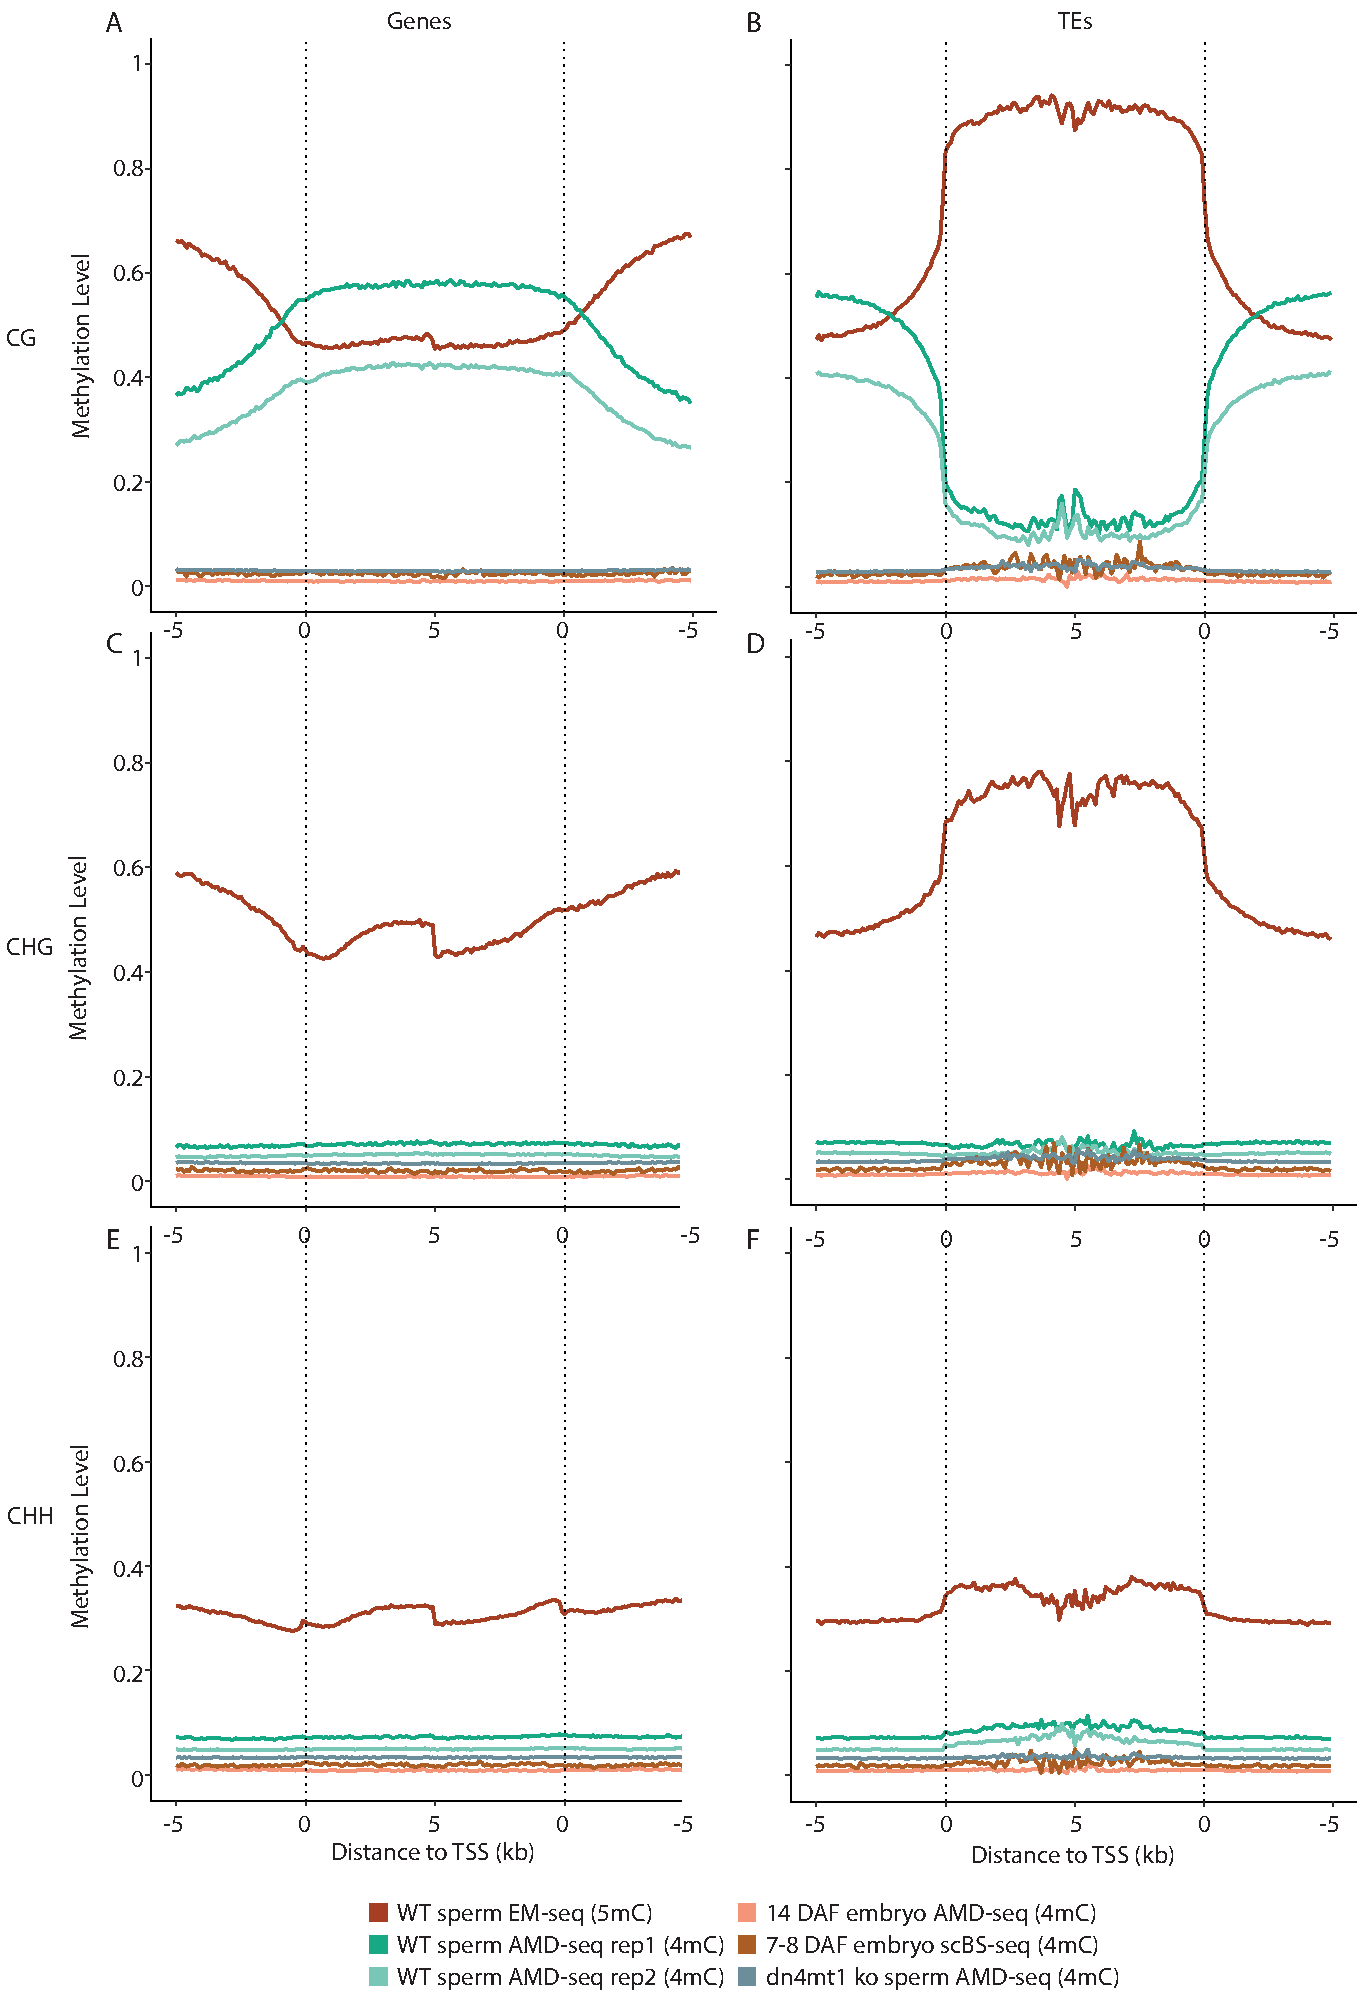
\includegraphics[width=1\textwidth]{Chapter3/Figs/Figure2_ends_analysis.pdf}
\caption{4mC methylation occurs in the CG context and is enriched in genic regions and outside TEs, while 5mC methylation is largely confined to TEs}
\label{fig:ends_analysis}
\captionsetup{font=small}
    \caption*{Panel showing 4mC and 5mC methylation across TEs (A) and Genes (B) in CG (first row), CHG (second row) and CHH (third row) sequence contexts in wild type sperm \textit{dn4mt1 sperm}, the embryo 7-8 and 14 days after fertilisation.}
\end{figure}

Thereafter, pre-meiotic embryos were dissected and sequenced using AMD-seq to establish a baseline for comparing early embryonic methylation patterns (Figure \ref{fig:ends_analysis}, 14 DAF embryos (orange)). The results confirmed the absence of 4mC methylation over genes or outside TEs (Table \ref{tab:methylation_levels}). Subsequently, 300 embryos at 7–8 DAF were collected, with 200 used for AMD-seq library construction and the remaining 100 embryos used for bisulfite sequencing libraries, pre-treated with APOBEC3A for an alternative 4mC sequencing method. Although AMD-seq is theoretically capable of handling low DNA input down to picogram levels \cite{idtdna_methylseq_kit}, this was not tested prior to sequencing the early embryos. The bisulfite sequencing protocol, on the other hand, was developed for low-input or single-cell sequencing and this has been robustly tested in our lab. Due to conversion issues, the AMD-seq library was not usable in this study. 

\begin{figure}[htbp!] 
\centering    
    \includegraphics[width=1\textwidth]{Chapter3/Figs/Figure3_H3K27me3.pdf}
\caption{H3K27me3 levels are elevated in the paternal genome and correlate with the presence of 5mC over genes}
\label{fig:h3k27me3}
\captionsetup{font=small}
    \caption*{Heatmaps showing the relative H3K27me3 levels in \textit{Marchantia} embryos over the genes and TEs in the paternal and maternal genomes. Data presented is from \cite{RN160}}
\end{figure}

At a surface level, the early embryo AMD-seq data indicated marginally higher 4mC methylation across genes compared to the mature AMD-seq library (Table \ref{tab:methylation_levels}). However, this increase fell within the error range of the experimental limitations (Table \ref{tab:methylation_levels}, "CHG and CHH levels of 4mC"). Moreover, the low levels of residual 4mC methylation did not display the expected distribution over genes and TEs, with no relative increase outside TEs or over genes. This suggests that the removal of paternal 4mC methylation may be essential for embryo development. However, starting with a methylation level of around 20\% in the zygote (based on the sperm AMD-seq levels), passive loss of 4mC by the 16–32 cell stage (7–8 days after fertilisation in our conditions) would result in very low residual 4mC methylation levels (Table \ref{tab:methylation_levels}). 

It has been previously demonstrated that during embryonic development the paternal genome is transcriptionally silenced and is marked with the repressive chromatin mark H3K27me3 mediated by maternally expressed Polycomb Repressive Complex 2 (PRC2) in the male pronucleus before the first zygotic division, approximately 3 days after fertilisation \cite{RN160}. This suggests the existence of a mechanism for paternal genome recognition, with blanket 4mC methylation being a potential candidate. To this end, visualizing H3K27me3 data across genes and TEs from this study confirms a paternal bias in the deposition of H3K27me3 (Figure \ref{fig:h3k27me3} right side). However, the pattern of H3K27me3 occupancy around gene and transposon transcription start sites does not align with the distribution of 4mC (Figure \ref{fig:h3k27me3} left side).

\begin{table}[htbp!]
\centering
\captionsetup{font=small}
\begin{tabular}{|p{5cm}|c|c|c||c|c|c|}
\hline
\multirow{2}{*}{\makecell{Methylation context}} & \multicolumn{3}{c||}{Overall} & \multicolumn{3}{c|}{Genes} \\
\cline{2-7}
 & CG & CHG & CHH & CG & CHG & CHH \\
\hline
WT sperm AMD seq rep1 & 0.467 & 0.071 & 0.075 & 0.559 & 0.071 & 0.072 \\
WT sperm AMD seq rep2 & 0.341 & 0.050 & 0.051 & 0.404 & 0.051 & 0.049 \\
dn4mt1 ko sperm & 0.031 & 0.035 & 0.033 & 0.029 & 0.034 & 0.033 \\
14 DAF embryo & 0.011 & 0.009 & 0.009 & 0.009 & 0.008 & 0.008 \\
7-8 DAF embryo & 0.027 & 0.021 & 0.019 & 0.025 & 0.020 & 0.020 \\
\hline
\multicolumn{7}{|l|}{Theoretical methylation levels} \\
\hline
Zygote & 0.202 & 0.030 & 0.031 & 0.241 & 0.030 & 0.030 \\
16 cell embryo  & 0.013 & 0.016 & 0.015 & 0.015 & 0.015 & 0.015 \\
32 cell embryo & 0.006 & 0.007 & 0.007 & 0.008 & 0.007 & 0.007 \\
\hline
\end{tabular}
\caption{Methylation levels across WT sperm, \textit{dn4mt1} sperm and the early embryo}
\label{tab:methylation_levels}
\end{table}


\section{\textit{De novo} methylation is deposited in genic regions specifically in the sporophyte of \textit{Marchantia}, targeted for methylation 24nt sRNAs through mismatches}

As described previously, \textit{de novo} methylation of genes in \textit{Arabidopsis} male meiocytes is mediated by 24nt sRNAs produced by HyperTE loci in the tapetum, the biogenesis of which is mediated by CLSY3 chromatin remodeller. Gene body methylation also exists specifically in the embryo and sporophyte of \textit{Marchantia} (Figure \ref{fig:SLM_examples}, data from Dr. James Walker). Sporophytic non-CG DMRs were determined as described before\cite{jimmythesis} and filtered to yield 221 methylated genic loci (MetGenes).

\begin{figure}[htbp!] 
\centering    
    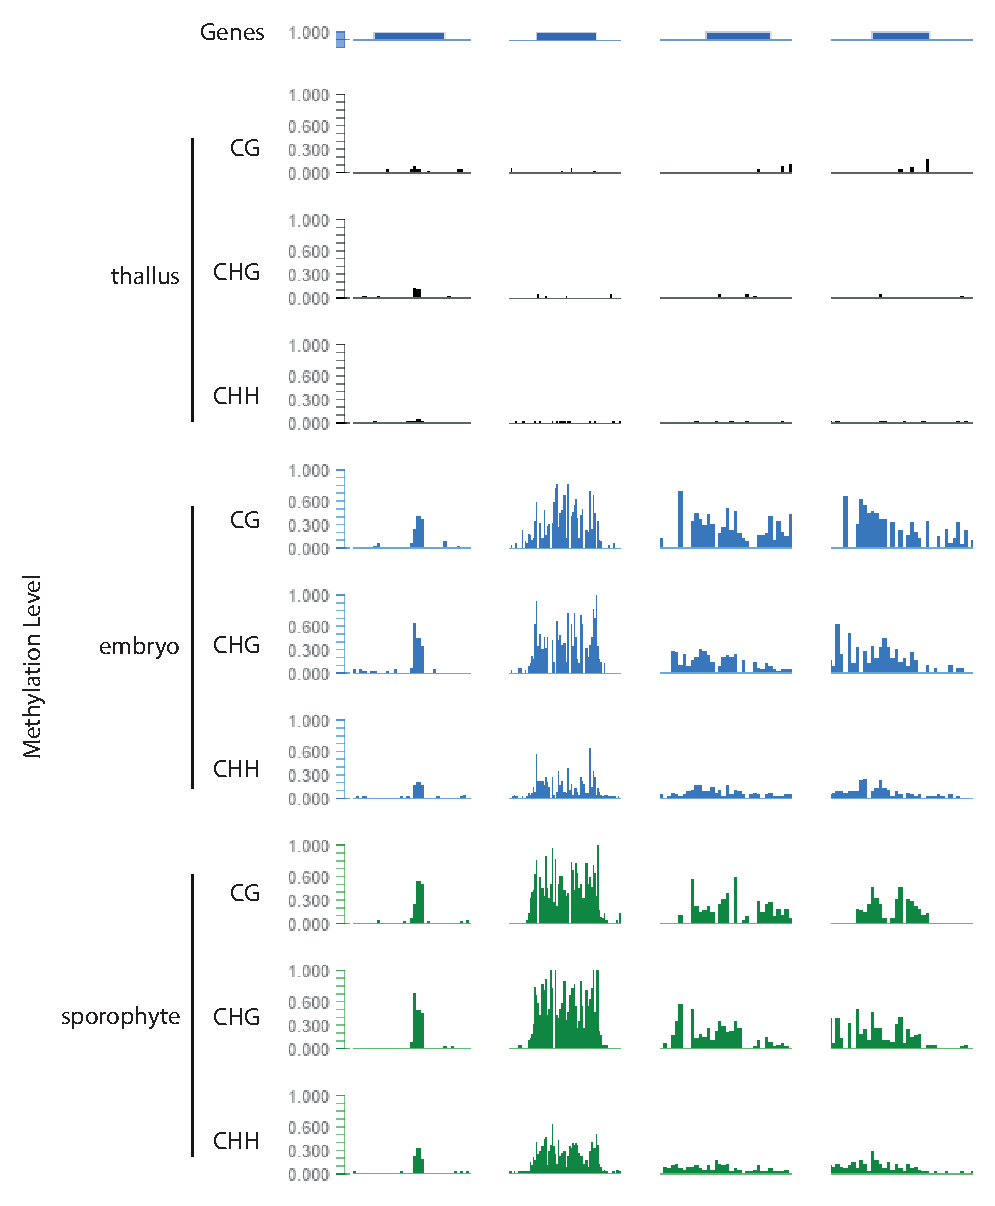
\includegraphics[width=1\textwidth]{Chapter3/Figs/Figure4_SLM_examples.pdf}
\caption{Sporophyte specific methylation exists in the embryos of \textit{Marchantia}}
\label{fig:SLM_examples}
\captionsetup{font=small}
    \caption*{CH, CHG and CHH methylation levels of genes which gain \textit{de novo} methylation specifically in the embyro and sporophyte of \textit{Marchantia}. Thallus (black), embryo (blue) and sporopyte (green)}
\end{figure}

With access to sRNA sequencing libraries from thallus, embryo, and sporophyte, the next step was to determine whether MetGenes could be targeted for methylation through mismatch targeting. To investigate this, the sRNA libraries were mapped to the reference genome, allowing for 0 and 3 mismatches. The sRNAs from the 3 mismatch dataset were then remapped onto the 0 mismatch dataset to identify identical sRNA sequences capable of targeting both TEs and genes with up to 3 mismatches. Reads overlapping MetGenes with 3 mismatches and TEs with 0 mismatches were then extracted. The resulting TE-MetGene pairs are visualised in Figure \ref{fig:SLM_targeting}A. It must be noted that one limitation of this method is the challenge of obtaining a comprehensive TE annotation for the gene model used in the study, as not all MetGenes could be paired with annotated TEs.

Indeed, when aligning the sequence of a source TE to its corresponding MetGene, an almost perfectly matching $\sim$160bp sequence was found (Figure \ref{fig:SLM_targeting}B). Notably, this alignment corresponds to the exact location where sporophyte-specific methylation is deposited within the MetGene (Figure \ref{fig:TE_SLM_pairs} red bar).

\begin{figure}[htbp!] 
\centering    
    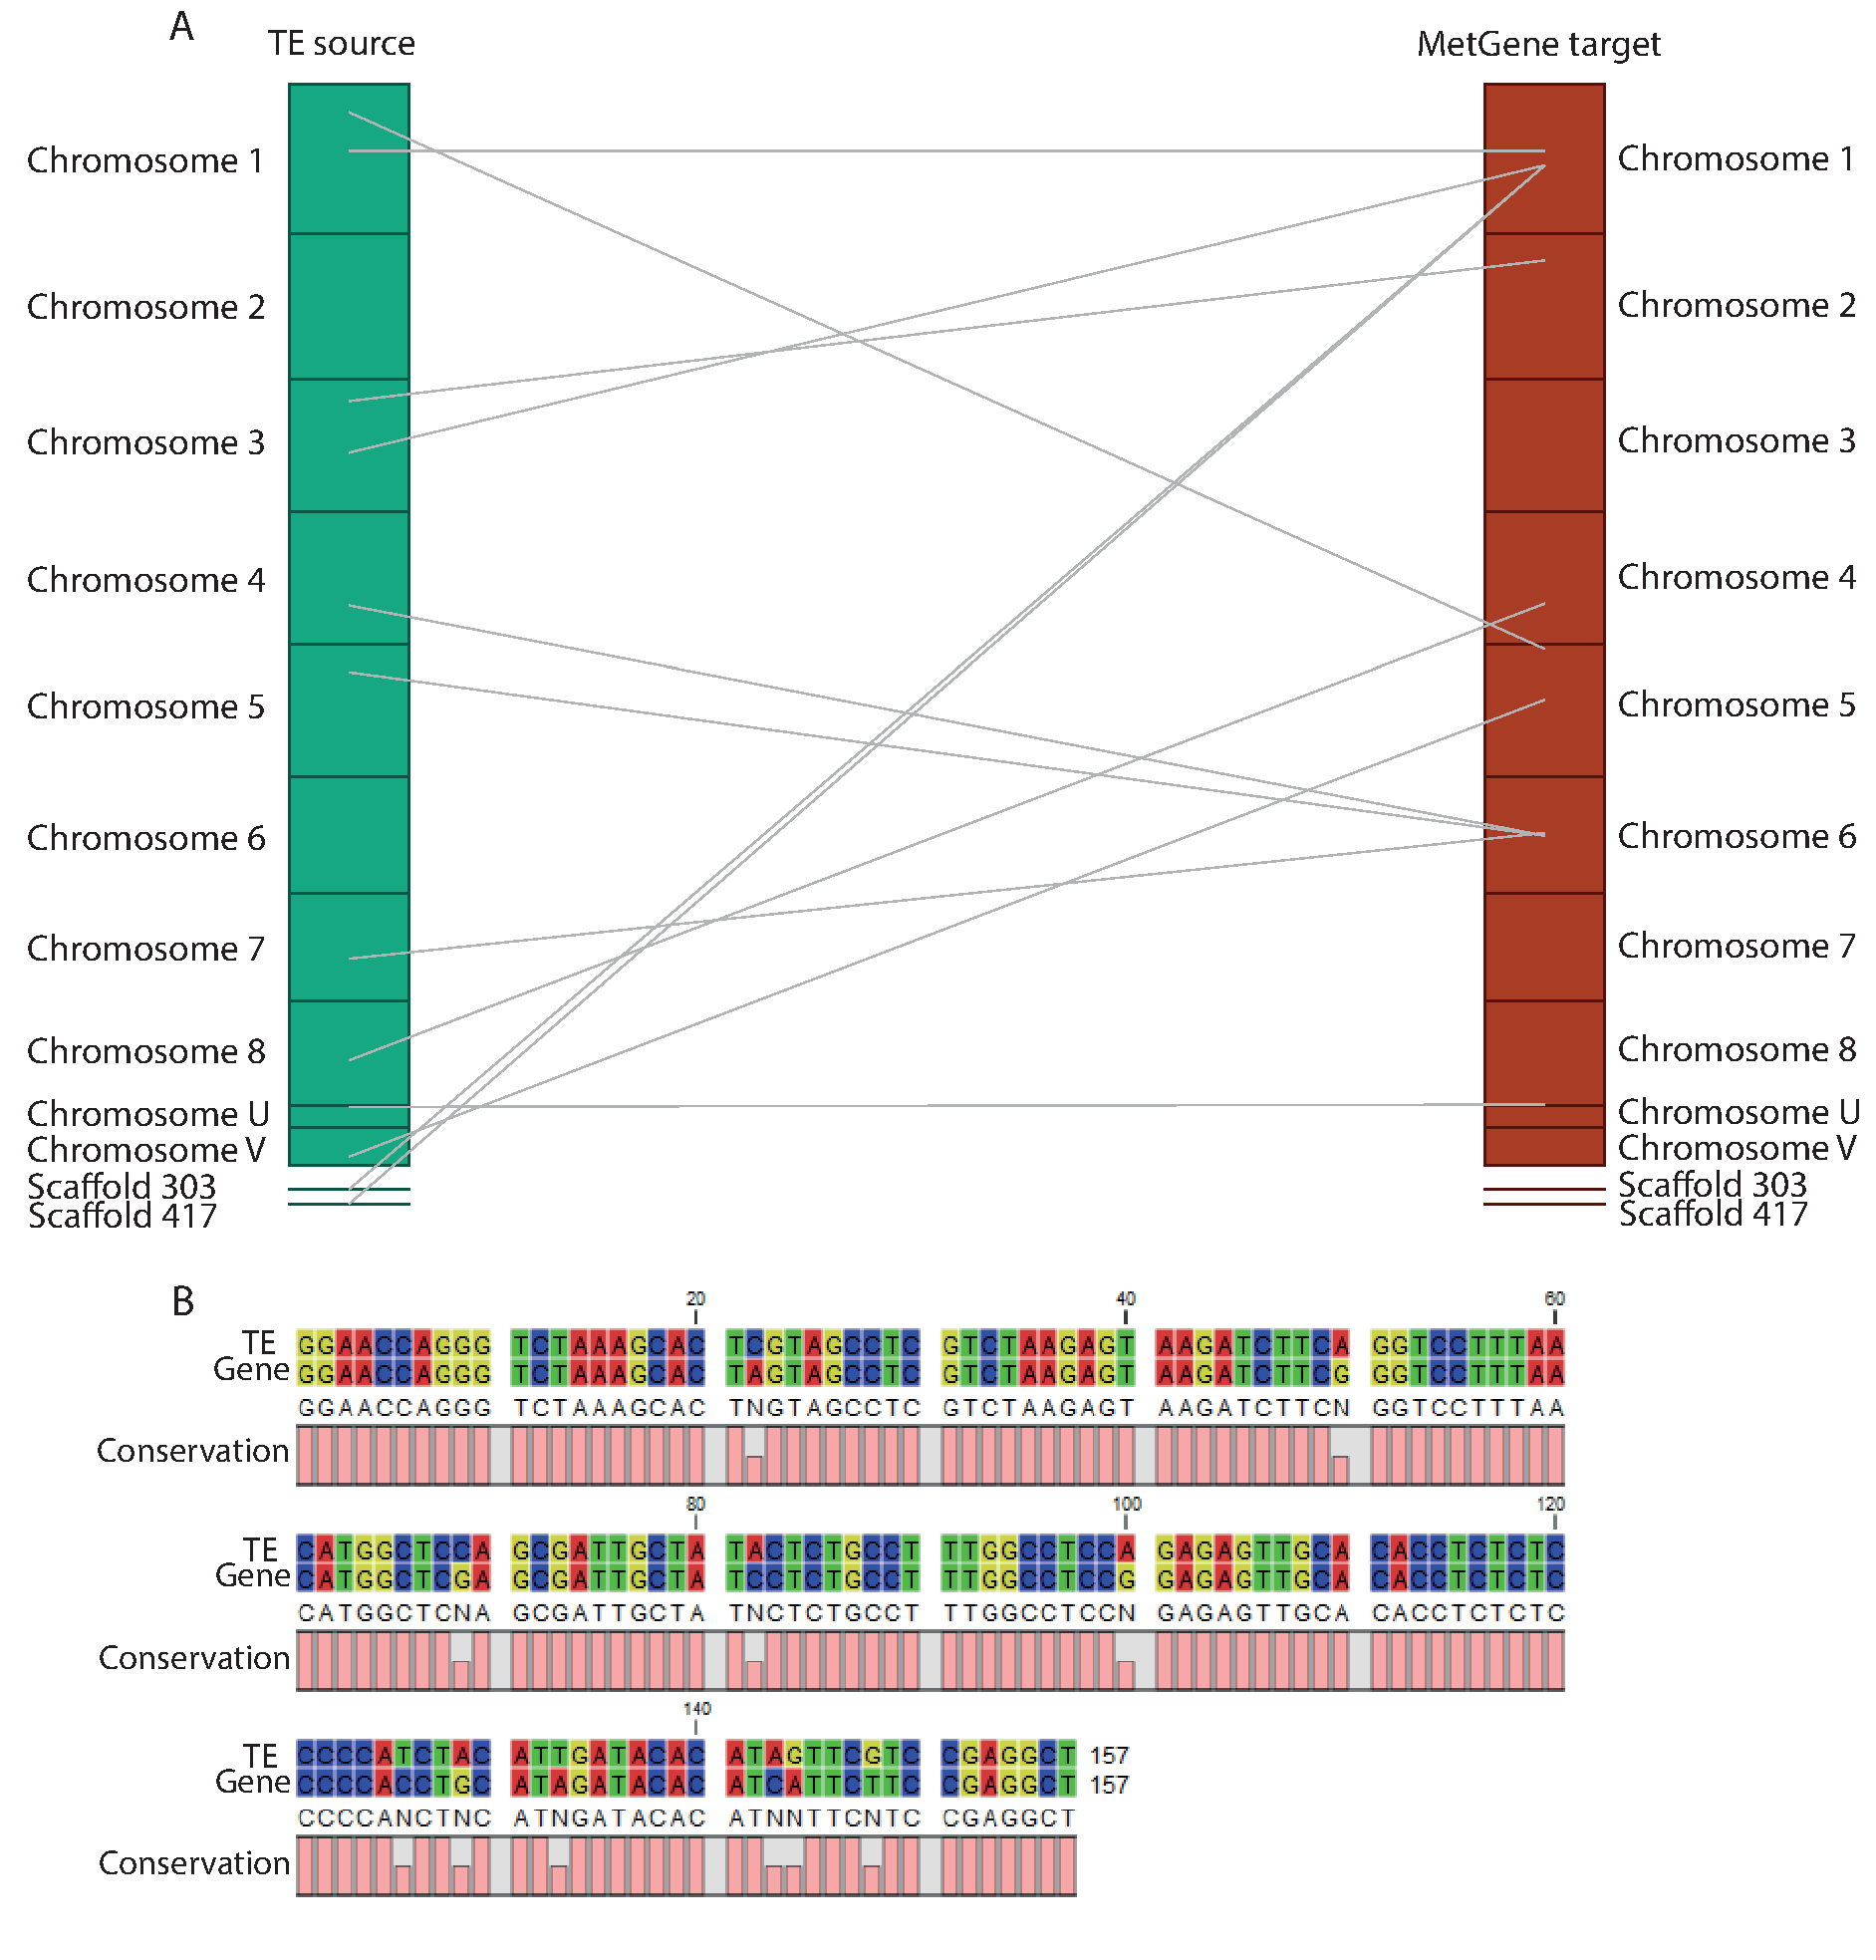
\includegraphics[width=1\textwidth]{Chapter3/Figs/Figure5_SLM_source_target.pdf}
\caption{TE loci produce 24nt sRNA that target genic loci for methylation with mismatch targeting}
\label{fig:SLM_targeting}
\captionsetup{font=small}
    \caption*{A)Locations of TE source loci (left, green) connected to genic target loci (right, brown) B) Alignment showing the sequence similarity between a TE-MetGene pair.}
\end{figure}

\begin{figure}[htbp!] 
\centering    
    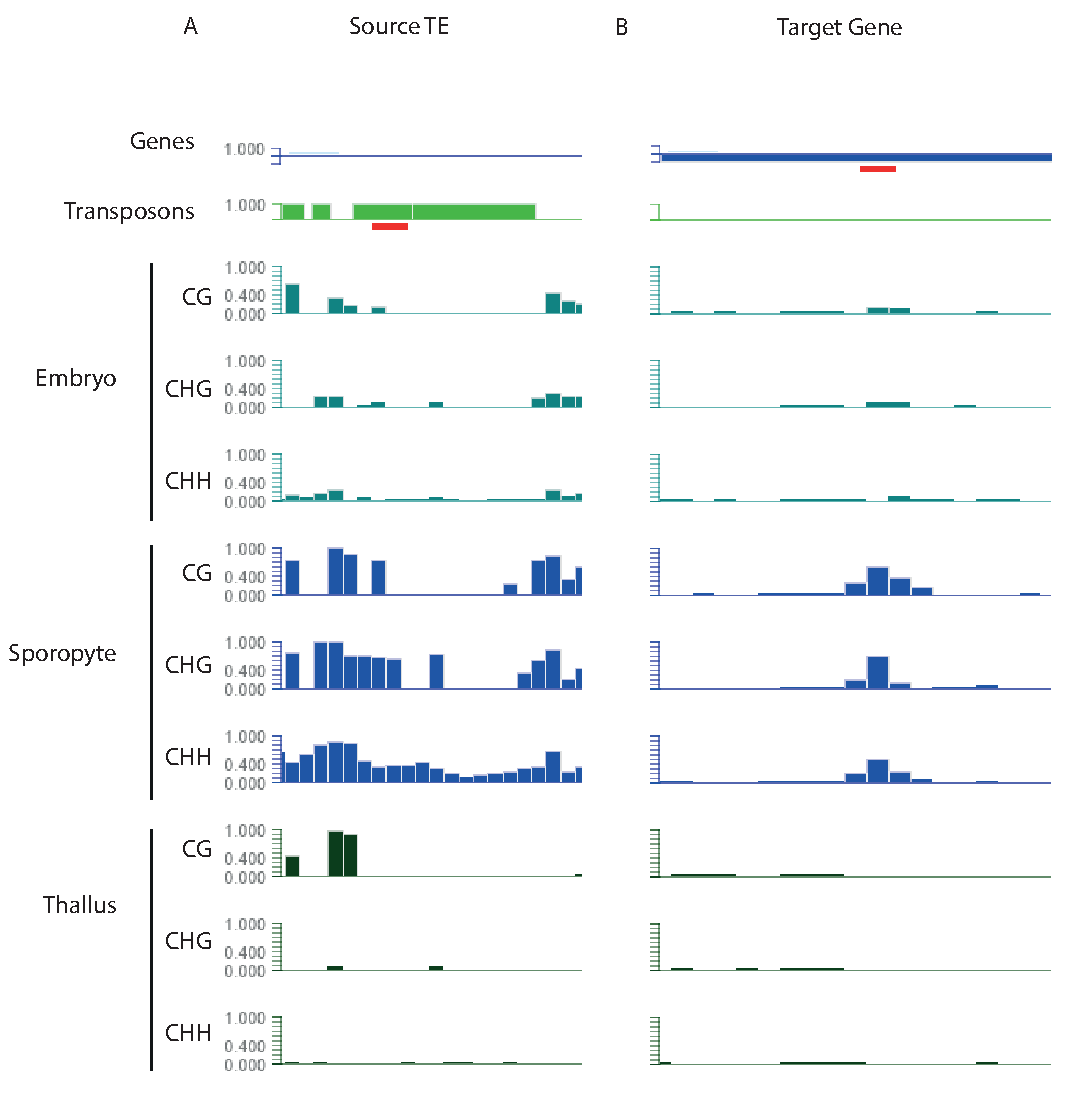
\includegraphics[width=1\textwidth]{Chapter3/Figs/Figure6_pairs_examples.pdf}
\caption{Example of a TE  source and MetGene target that gain methylation in the sporophyte}
\label{fig:TE_SLM_pairs}
\captionsetup{font=small}
    \caption*{Methylation levels in (A) TE source and (B) MetGene target pair in CG, CHG and CHH sequence contexts in embryo, (teal) sporophyte (blue) and thallus (green). Overlapping sequence highlighted with a red bar.}
\end{figure}

\section{Investigating the parental bias of sRNA production in \textit{Marchantia} embryos, sporophyte and thallus}

In the developing embryo, the paternal genome is deposited with H3K27me3, resulting in tight heterochromatic foci and transcriptional silencing \cite{RN160}. This raises the question whether sRNA production in the embryo and sporophyte is biased toward the maternal genome. To explore this, single nucleotide polymorphisms (SNPs) between Tak-1 (male) and Tak-2 (female) were analysed to calculate a SNP ratio. The sRNA sequencing libraries utilised were from the thallus, archegoniophore, and antheridiophore \cite{RN265} in addition to the libraries previously mentioned (Table \ref{ch3:workbyothers}).

The sRNA sequencing libraries were mapped to the reference genome with both no mismatches, and allowing one mismatch. Reads with mismatches at SNP positions were retained, as well as perfect matching sRNAs at SNP positions. A SNP ratio was calculated between the alternative and reference alleles for further analysis. Although several thousand SNP regions were initially covered, only those with at least 5 reads were retained to ensure robust results, which substantially reduced the number of SNP locations. 

Reads from archegoniophores displayed a SNP ratio near 1, as expected (Figure \ref{fig:sRNA_SNPs}A,B archegoniophore). Interestingly, in the early embryo, the data suggest a paternal bias in sRNA production, which shifts to a maternal bias in the sporophyte (Figure \ref{fig:sRNA_sizes}A,B embryo and sporophyte). As expected, the SNP ratio distribution in the embryo and sporophyte was less bimodal than in other tissues, indicating concurrent sRNA production from both genomes at multiple loci in the diploid phase. The thallus data seemed unreliable, with a surprising maternal bias despite originating from Tak-1 males \cite{RN265}.

\begin{figure}[htbp!] 
\centering    
    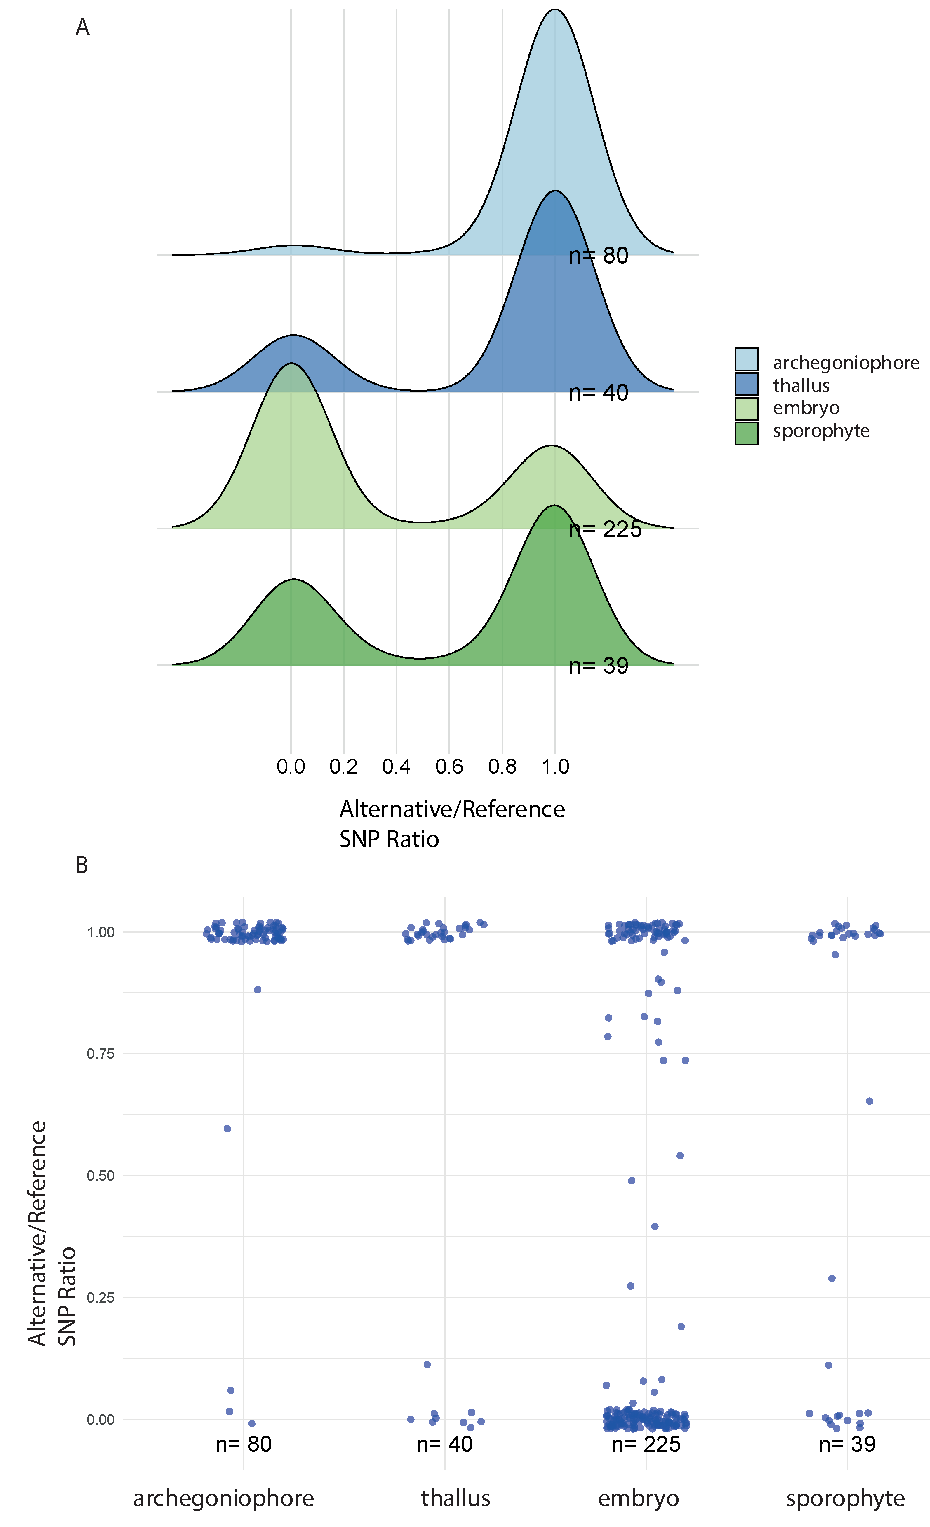
\includegraphics[width=0.9\textwidth]{Chapter3/Figs/Figure_sRNA_SNPs.pdf}
\caption{The association of sRNA sequences with parental genomes in different tissues}
\label{fig:sRNA_SNPs}
\captionsetup{font=small}
    \caption*{A) Ridge plot to show the SNP ratio of sRNAs in archegoniophores, thallus, embryo and sporophyte. Since the reference genome is Tak-1 a ratio close to 0 signifies a paternal bias, whilst a ratio close to 1 signifies a maternal bias. B) A density plot showing the SNP ratios at remaining SNP positions after stringent filtering conditions.}
\end{figure}

\clearpage

\section{Developing an effective method for visualising early embryonic development in \textit{Marchantia}}

The next objective was to determine whether the observed phenotype - where embryos fertilised with 4mC methylation mutants reach maturity earlier than wild type (Figure \ref{fig:burstpeak}) - was due to accelerated pronuclear fusion in the zygote, potentially caused by the absence of paternal 4mC. This led to the hypothesis that paternal 4mC may need to be actively removed before pronuclear fusion can occur.

As described earlier, staining live \textit{Marchantia} embryos proved challenging. A variety of fixing and staining methods were also trialled, including DAPI, Hoechst 33342 and ethidium bromide as staining dyes (the latter was used due to its small molecule size, which was expected to penetrate the fixed embryo), as well as different triton and formaldehyde concentrations and fixation times. Additionally, an egg cell reporter line was also tested (ECpro:MpSUN-GFP \cite{RN139}) showing strong expression; this faded after the first zygotic division, making it insufficient for visualizing early embryonic development (Figure \ref{fig:MpSUN}). 

Next, cell wall digestion enzymes such as cellulase and pectinase were trialled to improve dye penetration. While these enzymes increased dye uptake, they also compromised cell ultrastructure, hindering proper imaging of early embryonic development and cellular ultrastructure (Figure \ref{fig:enzyme_tests}). As a result, four constructs were designed to create constitutively expressing nuclear reporter lines. These constructs were driven by either the constitutive \textit{35S} promoter or the native \textit{elongation factor 1$\alpha$} (\textit{EF1$\alpha$}) promoter, fused with citrine or tdTomato, and tagged with a nuclear localisation signal (NLS) (Figures \ref{fig:35S_citrine_map}, \ref{fig:35S_tdTomato_map}, \ref{fig:EFalpha_citrine_map}, \ref{fig:EFalpha_tdTomato_map}). 

\begin{figure}[htbp!] 
\centering    
    \includegraphics[width=1\textwidth]{Chapter3/Figs/Figure7_Reporter_line_gemmae_screening.pdf}
\caption{Gemmae screening of constitutively expressed nuclear reporter lines}
\label{fig:gemma:screen}
\captionsetup{font=small}
    \caption*{Nuclear signal of tdTomato or citrine (second column, red or yellow respectively, white arrows) in gemmae, driven by either \textit{35S} constitutive promoter (first row) native constitutive promoter \textit{EF1$\alpha$} (second and third rows). Scale bar 10$\mu$m.}
\end{figure}

The constructs were initially transformed into Tak-1 thalli and selected in gemmae to avoid chimeric expression, resulting in the recovery of several independent lines from three of the four constructs (Figure \ref{fig:gemma:screen}). The constructs were then also transformed into sporelings from WTxWT, WTx\textit{dn4mt1} \#6 knockout and WTx\textit{dn4mt1} \#21 knockout crosses. Transformants were successfully recovered and screened for fluorescence expression in gemmae and antheridia (Figure \ref{fig:antheridia_screen}). Interestingly, while citrine reporter lines showed strong expression in gemmae, the strongest and most consistent expression was observed in transformants with the \textit{35S}::tdTomato-NLS and \textit{EF1$\alpha$}::tdTomato-NLS constructs. These lines were selected for crosses with wild-type female archegonia.

\begin{figure}[htbp!] 
\centering    
    \includegraphics[width=1\textwidth]{Chapter3/Figs/Figure8_Reporter_line_antheridia.pdf}
\caption{The tdTomato based nuclear reporter lines are expressed in the antheridia}
\label{fig:antheridia_screen}
\captionsetup{font=small}
    \caption*{Nuclear signal of tdTomato or citrine (second column, red or green respectively) in the antheridiophore, driven by either \textit{35S} constitutive promoter (first row) native constitutive promoter \textit{EF1$\alpha$} (second and third rows). Scale bar 10$\mu$m.}
\end{figure}

Unfortunately, despite strong expression in the antheridia, no nuclear reporter expression was detected in the developing zygote or embryo. This may be attributed to the previously mentioned shutdown of the paternal genome (Figure \ref{fig:malevsfemale}, first and second rows).  In response to this, wild-type female plants were recovered from the WTxWT \textit{35S}::tdTomato-NLS and  \textit{EF1$\alpha$}::tdTomato-NLS sporeling crosses (Figure \ref{fig:malevsfemale}, rows 3 and 4) with strong expression of their respective nuclear reporter lines. To improve clarity and fluorescence signal, a different clearing and staining method was employed, namely iTOMEI \cite{RN279}. In this protocol, the fixing component caprylyl sulfobetaine is able to clear chlorophyll without significantly quenching GFP (or other) fluorophores. After testing several environmental conditions, the best images were collected from 1\% FA fixation in PBS (pH 7.4) buffer for an hour, followed by clearing with caprylyl sulfobetaine for 24 hours (please see Materials and Methods for further details).

\begin{figure}[htbp!] 
\centering    
    \includegraphics[width=1\textwidth]{Chapter3/Figs/Figure9_reporter_line_malevsfemale.pdf}
\caption{Tak1 male nuclear reporter lines crossed to Tak2 females have no nuclear expression in the embryo}
\label{fig:malevsfemale}
\captionsetup{font=small}
    \caption*{Nuclear signal of tdTomato (second column, red, white arrows) in embryos crossing \textit{EF1$\alpha$}::tdTomato-NLS Tak1 male to WT Tak2 female, 3 days (first row) and 16 days (second row) after fertilisation. Expression of \textit{EF1$\alpha$}::tdTomato-NLS (third row) and  \textit{35S}::tdTomato-NLS (fourth row) in WT female thallus. Scale bar 10$\mu$m.}
\end{figure}

\section{Embryos crossed with 4mC methylation mutant sperm develop more rapidly than wild type during the first 7 days post-fertilisation}

Once mature archegoniophore-producing female plants were available from the selected \textit{35S}::tdTomato-NLS and \textit{EF1$\alpha$}::tdTomato-NLS lines, they were crossed with WT, \textit{dn4mt1} \#6 and \textit{dn4mt1} \#21 sperm. As before, the sperm was co-cultured with the archegoniophores for an hour, after which the developing embryos were dissected carefully, fixed and cleared daily, 1 to 7 days post-fertilisation. Due to the use of immature archegoniophores, embryos at 3 DAF were unfortunately unsuitable for imaging. In total, 338 embryos were imaged during the 7 days post-fertilisation and the developmental stages manually determined. 

\begin{figure}[htbp!] 
\centering    
    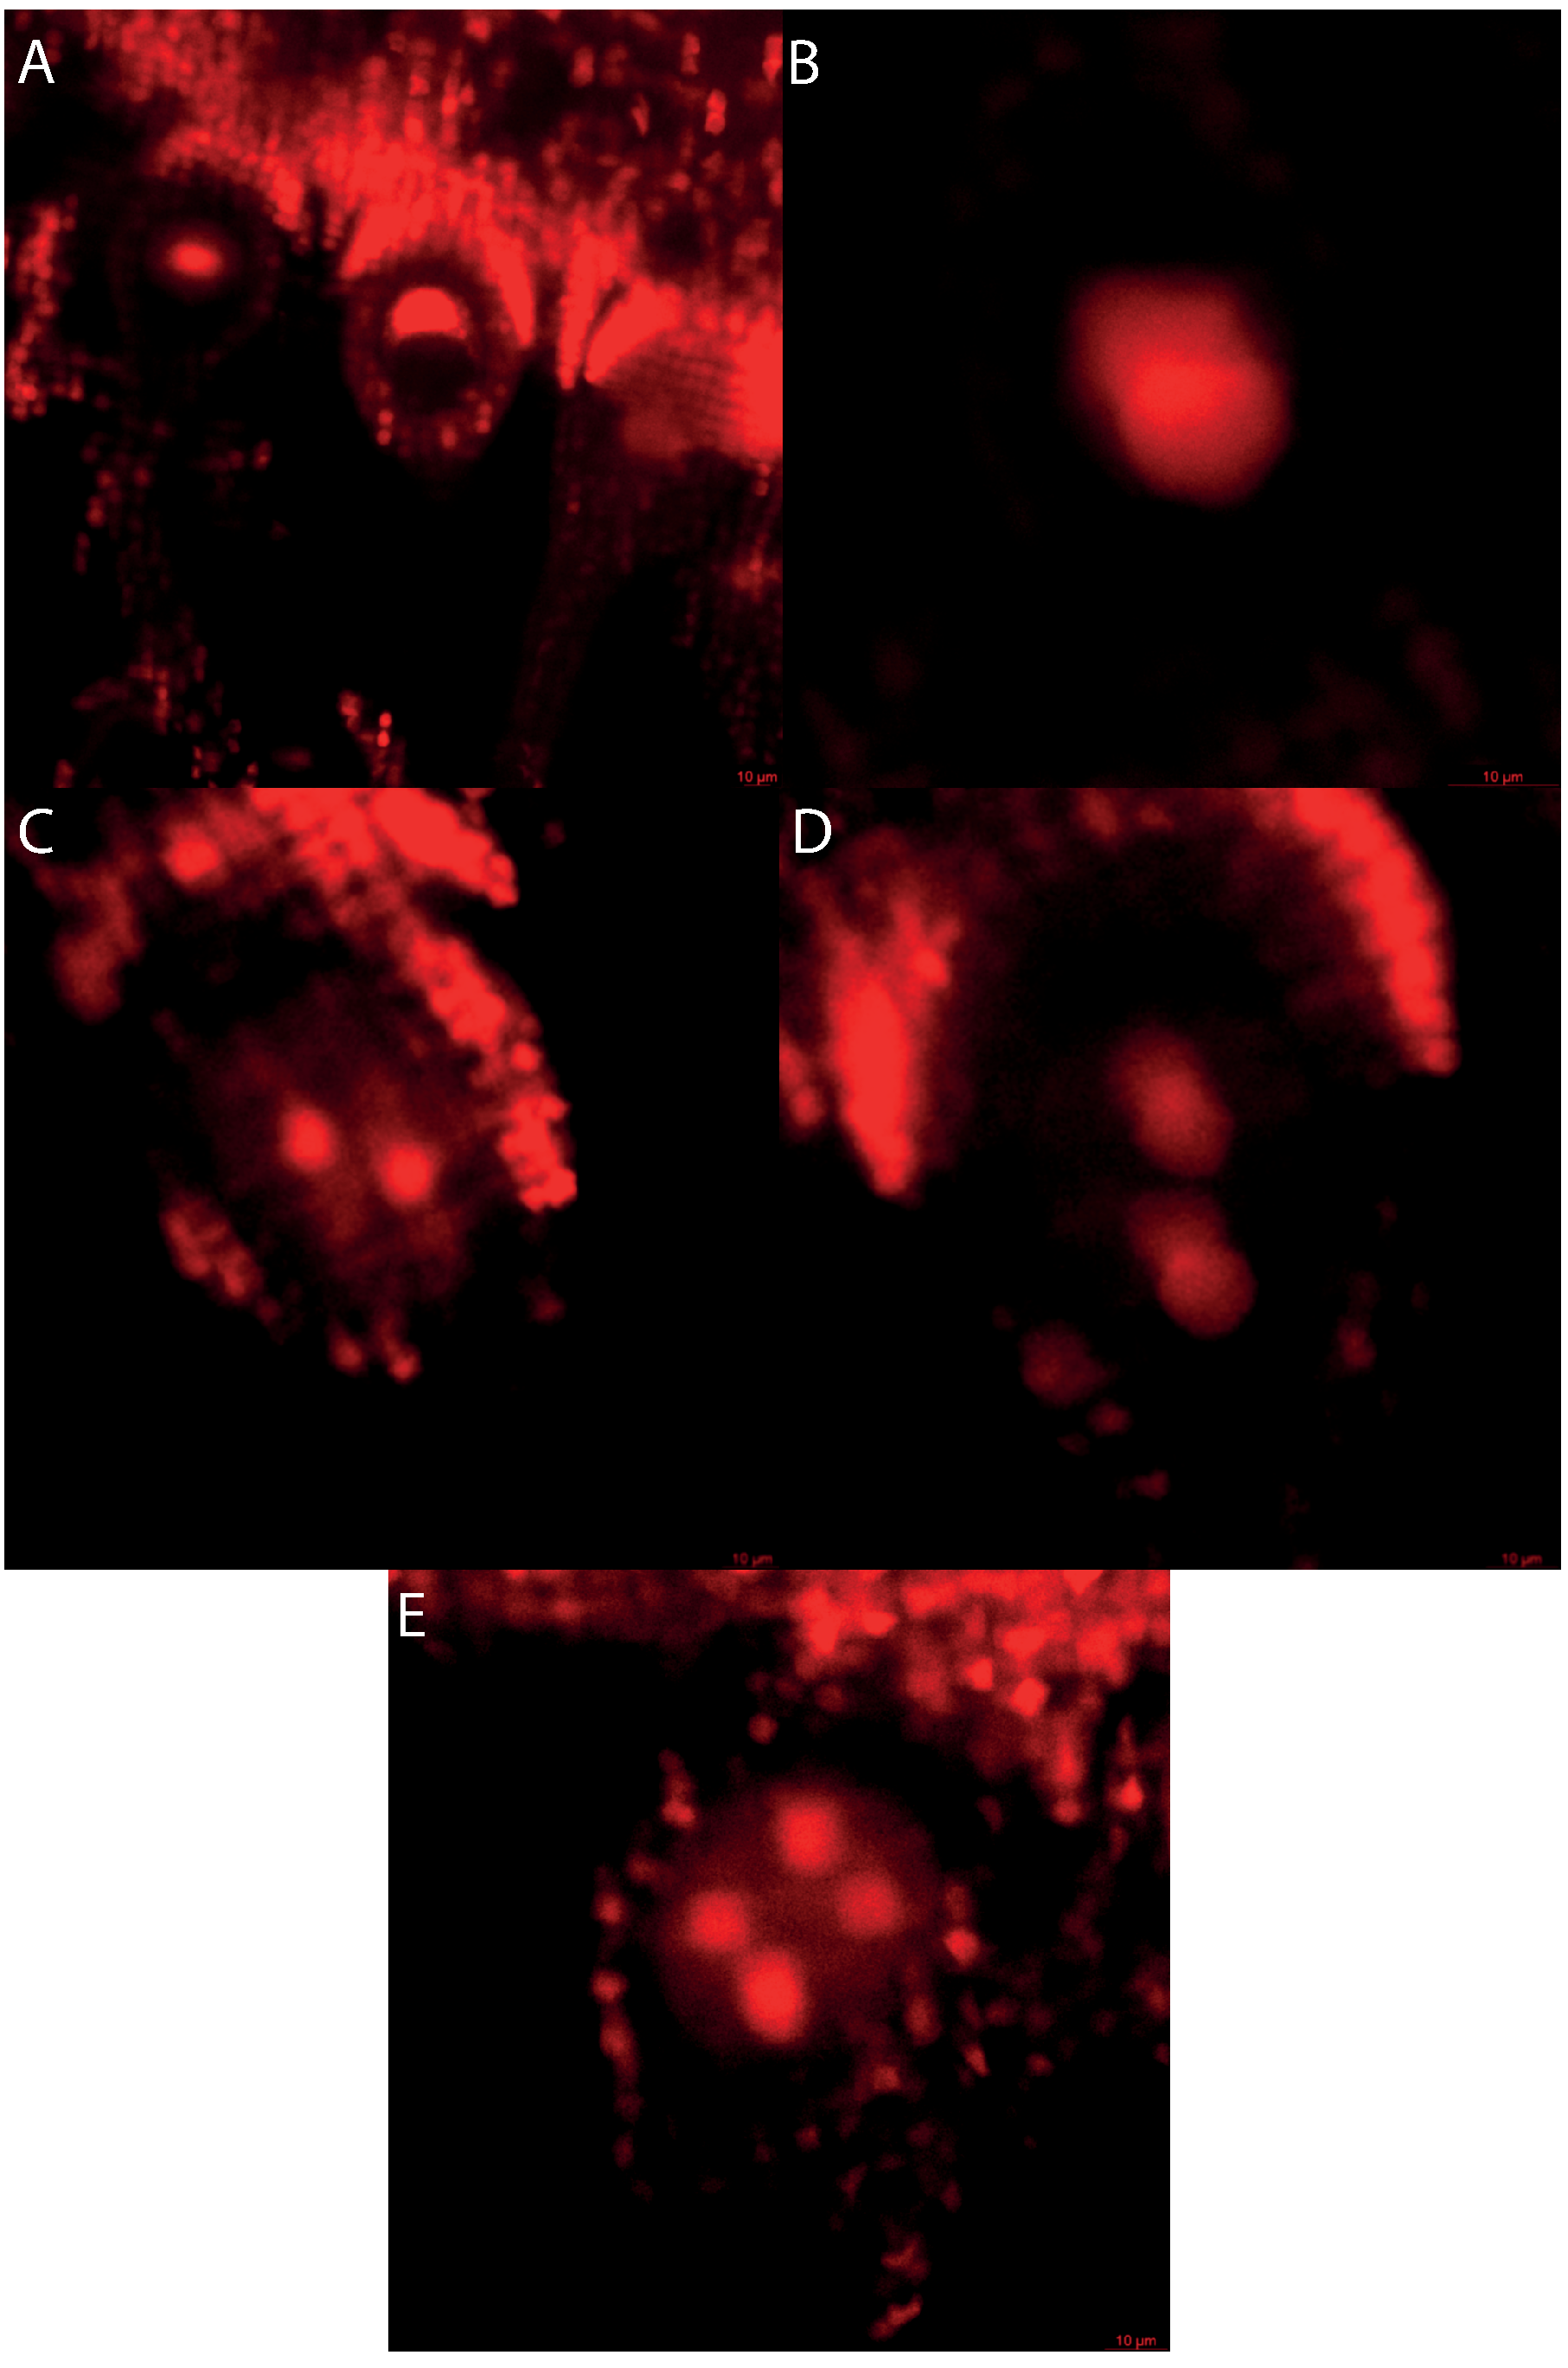
\includegraphics[width=1\textwidth]{Chapter3/Figs/Figure10_Developmental_stages.pdf}
\caption{Developmental stages of the early embryo (Tak1 male x \textit{EF1$\alpha$}::tdTomato-NLS WT female)}
\label{fig:dev_stages}
\captionsetup{font=small}
    \caption*{(A) Zygote (stage 1) (B) Zygote dividing (stage 2) (C) Two-cell stage (stage 3) (D) Two-cell embryo dividing (stage 4) (E) Four-cell stage (stage 5). Scale bar 10$\mu$m.}
\end{figure}

The developing embryo initially elongates through a transverse division, perpendicular to the archegonial axis, followed by a second vertical division to form four cells. The third division occurs at right angles to the previous ones, creating an octant of equal cells \cite{RN143,RN144}. Subsequent cell divisions progressively alter the embryo's initially circular shape. To further assess early cellular development, in addition to counting the nuclei, the transverse diameter of the embryonic venter cavity was measured. Interestingly, the mean transverse diameter of the embryos remained consistent and increased at a similar rate across all lines all until day 6, and between WT and \textit{dn4mt1} k.o. \#6 between days 6 and 7 (Figure \ref{fig:transverse_diameter}).

During the first two zygotic divisions, cells were frequently observed with multiple nuclei that had not yet undergone cytokinesis (Figure \ref{fig:dev_stages} B and D).  To facilitate tracking of cell development, these different stages were classified into distinct developmental phases:1. 1 nucleus 2. 2 nuclei, 1 cell, 3. 2 nuclei, 2 cells 4. 4 nuclei, 2 cells, 5. 4 nuclei, 4 cells, 6. 8 nuclei, 4 cells, 7. 8 nuclei, 8 cells, 8. 9–16 nuclei, 9. 16–25 nuclei, 10. 26–35 nuclei, 11. 36–45 nuclei, 12. 46–55 nuclei, 13. more than 55 nuclei.

Between days 1 and 5 post-fertilisation, embryos fertilised by either of the independent \textit{dn4mt1} knockout lines appeared to initiate division earlier than those fertilised by wild-type sperm. For example, by day 2, nearly all imaged cells in the \textit{dn4mt1} knockout lines had 2 nuclei, compared to fewer than a quarter in the wild type (Figure \ref{fig:nucleus_number} B,C).  

This trend persisted through day 4, where approximately a quarter of cells in the \textit{dn4mt1} knockout line \#6 had reached stage 4, while none of the wild-type cells had progressed that far. By day 5, the proportion of cells in various developmental stages became more synchronized across the genotypes. 

After day 5, the developmental differences between the wild type and the \textit{dn4mt1} knockout line \#6 were slight, but present: Some embryos from a \textit{dn4mt1} \#6 background reached stage 12 by day 7, whereas the most developed wild type embryos were slightly behind, at stage 11. It is also noteworthy that embryos from a  \textit{dn4mt1} \#6 knockout background displayed a proportion of cells arrested in stage 1 or 2, even at day 6 and day 7 (\ref{fig:nucleus_number} B,C). In contrast, embryos from the \textit{dn4mt1} knockout line \#21 continued to develop more rapidly than the wild type, the most advanced embryos reaching stage 13 by day 6 compared to stage 10 in wild-type (Figure \ref{fig:nucleus_number} B,C). 

Together, this data provides strong support that 4mC delays the onset of the first nuclear division, impacting long term developmental duration.


\begin{figure}[htbp!] 
\centering    
    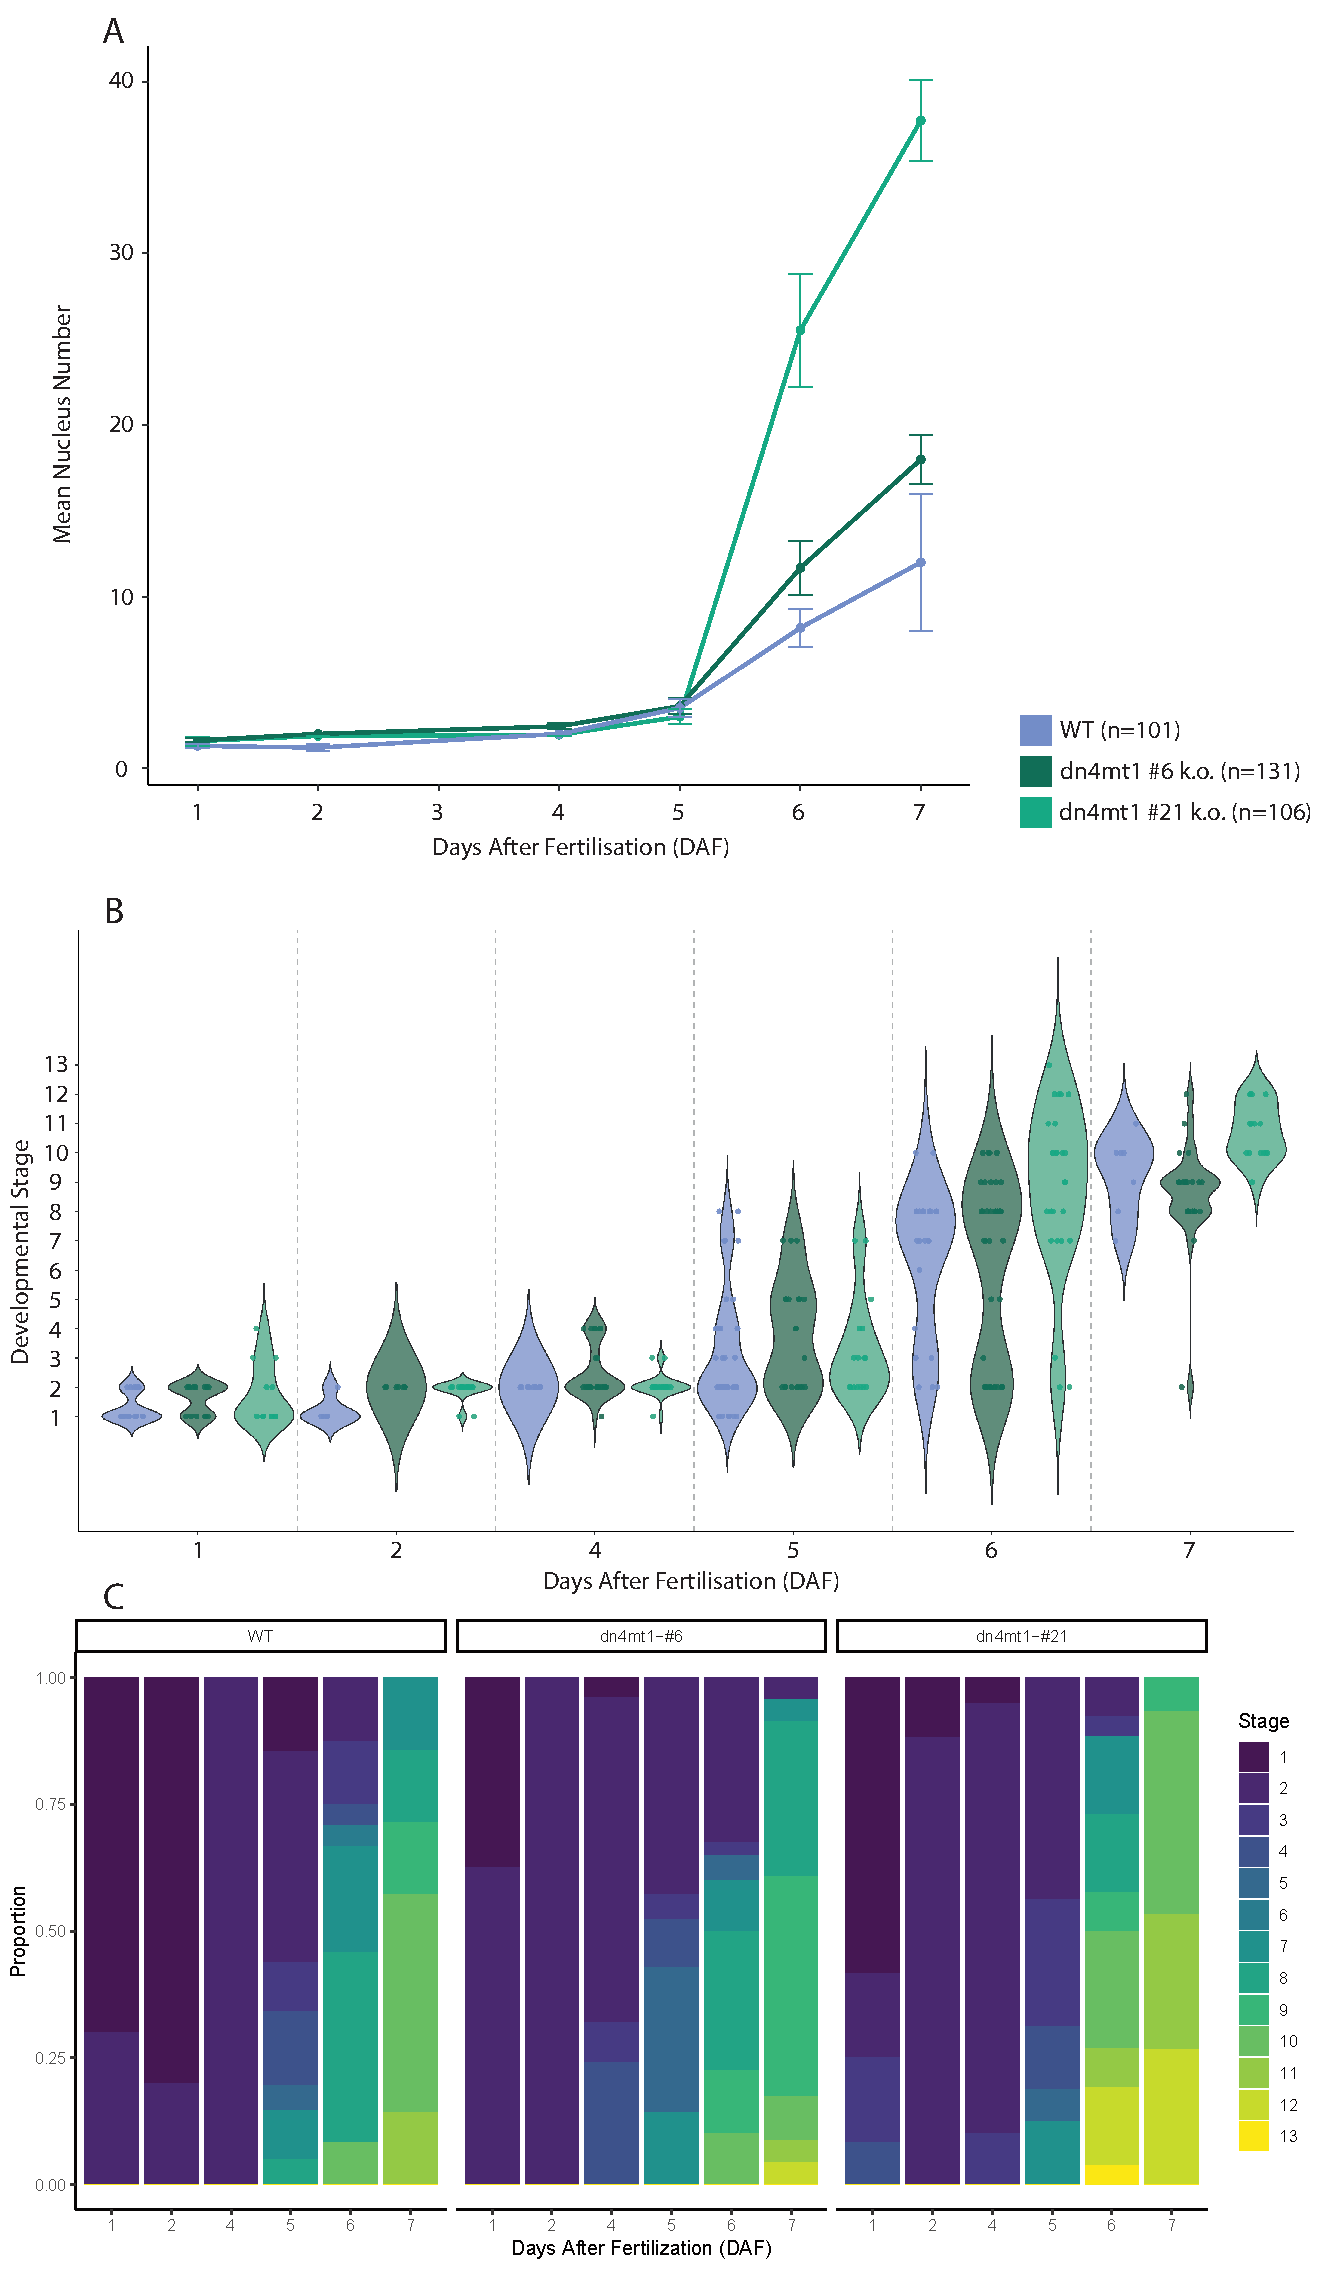
\includegraphics[width=0.95\textwidth]{Chapter3/Figs/Figure11_nucleus_number.pdf}
    \captionsetup{belowskip=0pt, aboveskip=0pt}
    \caption{Embryos fertilised by \textit{dn4mt1} knockout sperm develop more rapidly than WT}
    \label{fig:nucleus_number}
    \caption*{See next page for full caption.}
\end{figure}

\clearpage 

\FloatBarrier  % Prevents floating content from passing this point

% Full caption on the next page
\noindent\textbf{Full caption for Figure \ref{fig:nucleus_number}:} \\
A) Mean nucleus number of embryos from 1 to 7 days after fertilisation, fertilised by wild type (blue), \textit{dn4mt1} knockout \#6 (dark green), or \textit{dn4mt1} knockout \#21 (light green) sperm. 
B) Distribution of imaged embryos in different developmental stages from 1 to 7 days after fertilisation, categorised into distinct stages based on nuclei and cell numbers. 
Developmental stages: 1. 1 nucleus 2. 2 nuclei, 1 cell, 3. 2 nuclei, 2 cells 4. 4 nuclei, 2 cells, 5. 4 nuclei, 4 cells, 6. 8 nuclei, 4 cells, 7. 8 nuclei, 8 cells, 8. 9–16 nuclei, 9. 16–25 nuclei, 10. 26–35 nuclei, 11. 36–45 nuclei, 12. 46–55 nuclei, 13. 55< nuclei.
C) Proportion of embryos in developmental stages 1–7 days after fertilisation fertilised by wild type, \textit{dn4mt1} knockout \#6, or \textit{dn4mt1} knockout \#21 sperm.


\clearpage


\section{Discussion}

In angiosperms and other land plants, spermiogenesis involves chromatin compaction through the replacement of histones with sperm-specific histone variants \cite{RN283,RN284,RN285}. However, in \textit{Marchantia}, this process differs, as nucleosomes are replaced by protamines rather than histone variants. Consequently, DNA methylation becomes the primary heritable epigenetic mark in the paternal genome. This resembles the process in mammalian sperm, where the majority of histones are replaced by protamines, although some nucleosomes are retained \cite{RN282}. Following fertilisation, mammalian zygotes undergo global DNA demethylation, driven by  Ten-eleven translocation (TET) enzymes. This demethylation is crucial for transcriptional regulation, imprinting, and maintaining pluripotency in the early stages of development \cite{RN286,RN287}.

In \textit{Marchantia}, following fertilisation, protamines in the paternal pronucleus are replaced by histones, and H3K27me3 is deposited by a maternally expressed PRC2 complex \cite{RN160} specifically on paternal chromatin. This suggests a potential mechanism for paternal genome recognition, with paternal N4-methylcytosine blanket methylation emerging as a potential candidate.

However, when examining the distribution of H3K27me3 marks over genes and transposons, there is no clear alignment with 4mC occupancy (Figure \ref{fig:h3k27me3}). Furthermore, results from single cell bisulfite sequencing of early \textit{Marchantia} embryos revealed no evidence of paternal 4mC (Figure \ref{fig:ends_analysis}), Table \ref{tab:methylation_levels}). Additionally, Dr. Shujuan Xu confirmed that paternal H3K27me3 foci still form in embryos fertilised by \textit{dn4mt1} knockout sperm, 13 days after fertilisation (Figure \ref{fig:immuno}). These findings suggest that paternal genome recognition is not directly linked to blanket genome-wide 4mC methylation. However, it is important to consider that theoretical paternal 4mC trace levels in the embryo would likely be very low by 7-8 days post-fertilisation, assuming passive loss through cell division (Table \ref{tab:methylation_levels}). Further work is needed to optimise the protocol for low-input AMD-sequencing of \textit{Marchantia} embryos, as previous attempts were unsuccessful despite prior high-quality control datasets. To obtain a definitive answer,  developing reliable 4mC immunostaining and/or single-cell AMD-seq methods for zygotes or embryos at the 2-4 cell stage is essential, provided successful dissection at this early developmental stage can be achieved.

 Considering the shut-down of the paternal genome in the sporophyte, the possibility of sRNA production from the paternal genome became an intriguing question. Investigating whether there is a difference in sRNA production between the two parental genomes in the sporophyte, particularly in light of this potential suppression, revealed intriguing results. Initially, the sRNA data suggested a paternal bias in the embryo, which appeared to shift toward a maternal bias in the sporophyte, though substantial sRNA production was observed from both parental genomes (Figure \ref{fig:sRNA_SNPs}A,B). 
 
 Despite these findings, it is essential to acknowledge the limitations of this analysis. The male and female accessions used as the parental lines (Tak-1 and Tak-2) are asexually maintained in lab conditions, which means accumulated point mutations over time may significantly alter their genomic sequences. Indeed, at several SNP positions, bases other than the reference or alternative were observed across all datasets. Additionally, if Tak-1 had been crossed with other lines at any point, the resulting hybrid would exhibit a different SNP distribution from either parent.The unequal SNP distribution along different chromosomes further complicates the analysis, making these cultivars less suitable for complete genome coverage (Figure \ref{fig:chrom_ridge}). Moreover, the filtering steps applied to the sRNA data resulted in a limited number of data points, which restricts the ability to draw definitive conclusions. Ensuring the precise genetic background of the parental lines is therefore essential for accurate results, as is obtaining sufficient sequencing depths to definitively answer whether 24nt sRNAs are produced from both parental genomes in \textit{Marchantia} embryos. 
 
 Furthermore, exploring the distribution of H3K9me1 histone modifications on TEs in the mature embryo (as a proxy for locations that may be active in RdDM, as H3K9me2 has a direct interaction with SHH1, which recruits the Pol IV complex in \textit{Arabidopsis} \cite{RN116}) does not reveal a strong parental bias (Figure \ref{fig:h3k8me1}) \cite{RN160}. Nevertheless, addressing the limitations of the current dataset and producing a high-confidence, genetically distinct parental cross would provide valuable insights into the sRNA landscape of \textit{Marchantia} embryos. These results could then be cross-referenced with bisulfite sequencing data to draw more robust conclusions.

It has been previously noted that similar to genes hypermethylated in the male germline of \textit{Arabidopsis} (MetGenes), \textit{de novo} methylated genes are also present in the sporophyte of \textit{Marchantia} (Figure \ref{fig:SLM_examples} \cite{jimmythesis}). In \textit{Arabidopsis}, few perfectly matching sRNAs map directly to methylated MetGene regions. This observation led to the discovery that HyperTE-derived sRNAs target MetGene locations in meiocytes for methylation with up to three mismatches \cite{RN187} (Figure \ref{fig:At_0v3}). 

Building on this, once MetGene loci were identified in \textit{Marchantia} sporophytes, it was explored whether CHH methylation  at these genes could be targeted by sRNAs produced by TEs with high sequence homology. Although sequence homology between TE sources and target MetGenes was identified (Figure \ref{fig:TE_SLM_pairs}), a clear relationship between sRNA mismatch targeting and CHH methylation was not established. Mapping sRNAs to MetGene locations with up to 3 mismatches did not significantly increase the abundance of sRNAs at these locations (Figure \ref{fig:Mp_0v3}). 

Nevertheless, a mechanism must allow either the production of 24nt sRNAs and/or the targeting of TE-derived sRNAs for methylation at MetGenes specifically during the sporophyte stage. Further investigation is needed to verify this hypothetical causal relationship, including examining RdDM-associated protein variants uniquely expressed in the sporophyte and/or creating CRISPR/Cas9 knockout lines to mutate homologous sequences from the putative TE source to determine whether CHH methylation is abolished at the corresponding MetGene.

 Previous studies have shown that the mature pre-meiotic embryo loses all traces of paternal 4mC methylation \cite{RN189}. The removal of 4mC may be necessary for embryo development, as there is evidence that 4mC suppresses chromatin accessibility and transcription \cite{RN189}. There are two possible pathways through which paternal blanket 4mC methylation could be absent in the mature embryo or sporophyte.  One possibility is that after fertilisation, MpDN4MT1 is not expressed, or 4mC methylation is not actively maintained, leading to its gradual dilution through cell division. Alternatively, we can hypothesise that paternal 4mC methylation needs to be removed to allow pronuclear fusion. This hypothesis could explain the unusually long period required for \textit{Marchantia} embryos to undergo pronuclear fusion and complete the first zygotic division (up to 3–4 days after fertilisation) \cite{RN139}. Additionally, the accelerated sporophyte maturation observed in embryos fertilised by \textit{dn4mt1} mutant sperm, maturing up to 4 days earlier than wild-type embryos (Figure \ref{fig:burstpeak}), could support this explanation. In this scenario, MpROS1X (a DNA glycosylase encoded on the female chromosome) emerges as a potential candidate that could facilitate the removal of paternal blanket 4mC prior to pronuclear fusion.

When comparing early embryonic development between the two 4mC mutants and wild type, it is evident that zygotic divisions began earlier in both 4mC mutants than in the wild type (Figure \ref{fig:nucleus_number}B,C). Following this initial difference, all genotypes developed at a similar rate until day 5, with comparable nucleus numbers. However, after day 5, the 4mC mutants exhibited a sharp exponential increase in cell numbers over the next two days, while wild type embryos also underwent rapid cell division, but with a more gradual increase (Figure \ref{fig:nucleus_number}). Interestingly, despite the expectation that the wild type embryo's delayed early embryonic development would lead to a delayed entry into exponential growth compared to the 4mC mutants, both genotypes entered this phase simultaneously. The primary difference lay in the rate of cell proliferation, rather than the timing of its onset.

These findings suggest that 4mC removal may be required prior to pronuclear fusion. However, more detailed immunostaining or single-cell AMD-seq in the zygote is necessary, along with an investigation into the phenotypic effects of knocking out DNA demethylases, particularly MpROS1x. Additionally, it would be important to explore whether ROS1x possesses N4-methylcytosine glycosylase activity. Furthermore, despite accelerated embryonic development, the knockout of paternal 4mC appears to have a partial fertility cost, as some embryos in these knockouts exhibit delayed development or arrest (Figure \ref{fig:nucleus_number}B,C), a phenomenon observed in previous studies \cite{RN189}.

\clearpage

\section{Materials and Methods}

\subsection{Plant materials and growth conditions}

Male and female \textit{Marchantia polymorpha, L.} subsp. \textit{rudealis} accessions Takaragaike-1 (Tak-1, male) Takaragaike-2 (Tak-2, female) and Cam-2 (female) was used. The plants were grown on 1\% agar (Sigma-Aldrich), supplemented with ½ strength Gamborg's B5 medium. They were grown in a controlled environment chamber (Conviron) at 21°C with 70\% humidity under constant light with far-red light for induction of sexual reproduction, as described previously \cite{RN212,RN254}.

\subsection{Plasmid construction}

Four constructs were generated in total  using a Gateway\textregistered cloning system with either constitutive promoter \textit{35S} or the endogenous promoter \textit{EF1$\alpha$}, driving either citrine or tdTomato fluorophores with a nuclear localisation signal (NLS).

The insert for the BP reaction was amplified from plasmids pMpGWB115 (plasmid \#68569, Addgene) and pMpGWB116 (plasmid \#68570, Addgene) \cite{RN72} to get the citrine-NLS and tdTomato-NLS fragments respectively. The BP reactions were performed using the donor plasmid pDONR\texttrademark221 (Thermo Fisher (Invitrogen)). The LR reactions were performed using plasmids pMpGWB102 (plasmid \#68556, Addgene) and pMpGWB103 (plasmid \#68557, Addgene)\cite{RN72} as the backbones for the \textit{35S} and \textit{EF1$\alpha$} promoter driven expression clones respectively. These constructs yielded the final 4 expression clones: MpGWB102(p\textit{35S})-citrine-NLS, MpGWB102(p\textit{35S})-tdTomato-NLS, MpGWB103(p\textit{EF1$\alpha$})-citrine-NLS, MpGWB103(p\textit{EF1$\alpha$})-tdTomato-NLS. The constructs were transformed into \textit{Escherichia  coli}, purified and the sequence confirmed, followed by transformation into \textit{Agrobacterium tumefaciens} strain MP90.

The primers used and plasmid maps are available in Appendix B Table \ref{table:reporter_primers} and Figures \ref{fig:35S_citrine_map}, \ref{fig:35S_tdTomato_map}, \ref{fig:EFalpha_citrine_map} and \ref{fig:EFalpha_tdTomato_map}.

\subsection{Thallus and sporeling transformation}

For thallus transformation, Tak-1 gemmae were grown for 18-20 days in a controlled environment chamber (Conviron) at 21°C with 70\% humidity under constant light on 1.2\% agar (Sigma-Aldrich), supplemented with ½ strength Gamborg's B5 medium. Following 18-20 days, thalli were cut and the basal fragments regenerated on plates supplemented with 1\% sucrose for 3 days. The thalli were then co-cultured with \textit{Agrobacteria} (strain MP90) in 0M51C liquid media for 3 days and transformants selected on 1\% agar (Sigma-Aldrich) supplemented with 10 $\mu$g/mL hygromycin and 120 $\mu$g/mL cefotaxime for several weeks. Fluorescent gemmae were selected from transformant thalli and regenerated again to avoid chimeric plants\cite{RN147}. 

For sporeling transformation, sporangia of backgrounds WT x WT, WT x Mp\textit{dn4mt1} \#6 and T x Mp\textit{dn4mt1} \#21 were sterilised in 1mL of Milton's sterilising solution on a rotating shaker for 20 minutes. The spores were pelleted and washed with sterile water twice. The sterilised spore suspension was added into 25mL 0M51C liquid medium and the flasks were incubated in a growth chamber with constant light at 1500-2000 lux, 23 °C for 5-7 days. Induced \textit{Agrobacterial} cultures (strain MP90) containing each vector was co-cultivated with the sporelings for 2 days on a rotating shaker. the spore culture was strained and washed with sterile water and transformants were selected on 1\% agar (Sigma-Aldrich) supplemented with 10 $\mu$g/mL hygromycin and 120 $\mu$g/mL cefotaxime for several weeks\cite{RN146}.

\subsection{Semi in vitro culture and crossing}

Semi in vitro culture and crossing was performed as described previously\cite{RN139}. Briefly, mature female archegonia were collected into 5mL tubes containing 3mL water and co-cultured with male antheridia for 1 hour under white light at 22°C. The fertilised archegonia were then washed and incubated in 5mL tubes containing 3mL of fresh water under white light at 22°C until observation.

\subsection{Microscopy} 

The archegoniophores were collected for dissection and imaging and were either observed live or were fixed for imaging. For live cell imaging, rows of archegonia were manually dissected from the base of digitate rays and the embryo dissected out using micro knives or double lancet sapphire surgical knives (Fine Science Tools, World Precision Instruments) collected on cavity slides (BRAND\textregistered) and washed twice with 1x PBS to remove any maternal tissue. They were then stained with DAPI for 5 mins and briefly vacuum infiltrated and observed using slides with imaging spacers (Thermo Scientific™ Gene Frame) or on cavity slides \cite{RN139}. 

For observing developmental synchronicity and the Mp\textit{dn4mt1} early developmental phenotype,  rows of archegonia were manually dissected from the base of digitate rays removing involucres. The fluorescent samples were fixed and stained using the iTOMEI protocol \cite{RN148} using 1\% FA fixation for an hour in 1X PBS (pH 7.4) followed by clearning (20\% caprylyl sulfobetaine for 24 hours) and mounted in iohexol with imaging spacers (Thermo Scientific™ Gene Frame). The embryo/egg cells were imaged using a Leica SP8X confocal microscope.

\subsection{AMD-sequencing and bisulfite-sequencing library construction}

Dissected Tak-1 x Cam-2 embryos were used to construct 4mC AMD-seq libraries using the xGen™ Methyl-Sequencing DNA Library Preparation Kit (IDT, 10009860) after treatment of sheared DNA with APOBEC3A (NEB \#E7120S), following manufacturer’s instructions. In parallel, a bisulfite sequencing library was also contructed after APOBEC3A treatment using the Imprint\textregistered DNA Modification Kit (Sigma-Aldrich, MOD50)


\subsection{Imaging analysis}

The collected images were analysed in Fiji (ImageJ) \cite{RN266}. The macro was created to automate the image analysis steps, whereby a maximum Z projection was applied to the 3D image stack and a Gaussian blur was applied. The selected region on interest (the embryo) was then masked and a local contrast was then enhanced using the CLAHE plugin, and nuclei were counted manually in the resulting images using the ROI Manager. The resulting data was visualised in R using the ggplot2 package.

\subsection{Determination of MetGenes}

MetGene locations were defined using parameters previously described \cite{jimmythesis}. Briefly, bisulfite sequencing reads were mapped using a custom mapping script based on Bismark \cite{RN229}, and fractional methylation (50bp windows) was determined for each sample in the  CG, CHG and CHH contexts using MethylDackel v0.4.0 and custom scripts. Windows were selected where C-methylation was greater than 0.05 and adjacent windows merged if they occured within 200bp. The methylation difference in each context was determined between the sporophyte and thallus, and retained according to these filtering criteria: Islands greater than 99bp; significantly different non-CG metylation between sporophyte and thallus (Fisher's exact test p<0.001); CG, CHG, CHH and non-CG difference between sporophyte and thallus bigger than 0, 0.05, 0.1 and 0.3 respectively. The final filtering step kept islands that had less than 0.1 CG methylation in the thallus and overlapped genic regions. The final list yielded 221 DMRs.

\subsection{Histone analysis}

CUT\&RUN reads were were processed using SAMtools v1.9 \cite{RN174}, BEDtools v2.27.1 \cite{RN90} and Picard v2.18.27 \cite{RN173} then mapped to the Takv6.1 genome \cite{RN179} using bwa v0.7.17 \cite{RN182}. To distinguish between maternal and paternal sequencing reads, a SNP analysis was conducted. SNPs were called using gatk v4.0.1.2 \cite{RN177} wherein the SNPs between the parental Tak-1 and Cam-2 were replaced with Ns. The parental reads were assigned using SNPSplit v0.3.4 \cite{RN178} and counts for each parental genome were calculated using SAMtools v1.9 and BEDTools v2.27.1. Please see reference \cite{RN160}  for a detailed description of the pipeline. 

\subsection{sRNA analysis}

The sRNA reads were processed using Trim Galore! v0.4.2 \cite{trim_galore}, and mapped using bowtie v1.0.1 \cite{RN89} allowing for 0 or up to 3 mismatches with the -v option. For the TE-MetGene matching analysis, the resulting BAM files were converted to fasta files using custom awk scripts. The reads were once again mapped using bowtie, with no mismatches. Finally the resulting reads in the BAM files were queried against original genome locations using custom awk scripts, and the resulting file was filtered by MetGene locations with BEDtools v2.27.0.

For the sRNA SNP analysis, a SNP file was created using the method described above but this time using Tak-1 and Tak-2 as the parental genomes. 24nt reads overlapping MetGene locations with 0 or 1 mismatches were filtered using BEDtools v2.27.0 and were kept if they overlapped SNP positions. From the 1 mismatches dataset, only reads that mismatched exactly at the SNP positions were kept to prevent reads that mismatch elsewhere but also covering SNP positions from biasing the data. The perfect matching dataset was downsampled to prevent this much larger dataset from biasing the data. The reference, alternative or other bases were counted at each SNP position using SAMtools mpileup and this dataset was imported to R for visualisation in R using the ggplot, ggpubr and ggridges packages. Please find all scripts used at \href{https://github.com/talasjudit}{my personal GitHub page}.


